% !TeX spellcheck = pt_BR
%%%%%%%%%%%%%%%%%%%%%%%%%%%%%%%%%%%%%%%%%%%%%%%%%%%%%%%%%%%%%%%%%%%%%%%%%%%%%%%%%%%%%%%%%%%%%%%%
%                                                                                              %
%                             Definicao para a classe Artigo                                   %
%                                                                                              %
%%%%%%%%%%%%%%%%%%%%%%%%%%%%%%%%%%%%%%%%%%%%%%%%%%%%%%%%%%%%%%%%%%%%%%%%%%%%%%%%%%%%%%%%%%%%%%%%

\documentclass[portugues, brazil, a4paper,12pt]{article}
\bibliographystyle{plain}

%%%%%%%%%%%%%%%%%%%%%%%%%%%%%%%%%%%%%%%%%%%%%%%%%%%%%%%%%%%%%%%%%%%%%%%%%%%%%%%%%%%%%%%%%%%%%%%%
%                                                                                              %
%                       Pacotes a utilizar na compilacao do documento                          %
%                                                                                              %
%%%%%%%%%%%%%%%%%%%%%%%%%%%%%%%%%%%%%%%%%%%%%%%%%%%%%%%%%%%%%%%%%%%%%%%%%%%%%%%%%%%%%%%%%%%%%%%%

\usepackage[brazil]{babel}
\usepackage{graphicx}
\usepackage{geometry}
\usepackage[utf8]{inputenc}
\usepackage[T1]{fontenc}
\usepackage{algorithm}
\usepackage{color}
\usepackage{minted}
%\usepackage{algorithmic}
\usepackage[noend]{algpseudocode}
\usepackage{epstopdf}
\usepackage{hyperref}
\usepackage{todonotes}
\usepackage{amsmath}
\usepackage{verbatim}
\usepackage{gensymb}
\usepackage{subfigure}

\hypersetup{
    colorlinks,
    citecolor=black,
    filecolor=black,
    linkcolor=black,
    urlcolor=black
}


\title{Seguidor de Linha Controlado}

\makeatletter
\renewcommand{\paragraph}{\@startsection{paragraph}{4}{0ex}%
   {-3.25ex plus -1ex minus -0.2ex}%
   {1.5ex plus 0.2ex}%
   {\normalfont\normalsize\bfseries}}
\makeatother

\stepcounter{secnumdepth}
\stepcounter{tocdepth}

%%%%%%%%%%%%%%%%%%%%%%%%%%%%%%%%%%%%%%%%%%%%%%%%%%%%%%%%%%%%%%%%%%%%%%%%%%%%%%%%%%%%%%%%%%%%%%%%
%                                                                                              %
%                       Configuracao dos pacotes utilizados no doc.                            %
%                                                                                              %
%%%%%%%%%%%%%%%%%%%%%%%%%%%%%%%%%%%%%%%%%%%%%%%%%%%%%%%%%%%%%%%%%%%%%%%%%%%%%%%%%%%%%%%%%%%%%%%%

\geometry{a4paper,left=3cm,right=3cm,top=2.5cm,bottom=2.93cm}


%%%%%%%%%%%%%%%%%%%%%%%%%%%%%%%%%%%%%%%%%%%%%%%%%%%%%%%%%%%%%%%%%%%%%%%%%%%%%%%%%%%%%%%%%%%%%%%%
%                                                                                              %
%                             Capa do relatorio tecnico                                        %
%                                                                                              %
%%%%%%%%%%%%%%%%%%%%%%%%%%%%%%%%%%%%%%%%%%%%%%%%%%%%%%%%%%%%%%%%%%%%%%%%%%%%%%%%%%%%%%%%%%%%%%%%

\begin{document}

\begin{titlepage}

  \vfill

	\begin{figure}[H]
	\centering
		
\includegraphics[scale=0.15]{img/logo-ufop.jpg}
	\end{figure}
  \vfill

  \begin{center}
    \begin{Large}
      \textbf{UNIVERSIDADE FEDERAL DE OURO PRETO}
    \end{Large}
  \end{center}

  \begin{center}
    \begin{large}
      \textbf{Mestrado em Ciência da Computação} \\[1.4cm]
    \end{large}
  \end{center}

  \vfill

  \begin{center}
    \begin{large}
      \textbf{Relatório de Projeto e Desenvolvimento do Carro Robô Seguidor de Linha Utilizando Controle Proporcional}
    \end{large}
  \end{center}

  \vfill

  \begin{center}
    \begin{large}
      Disciplina: \\
		Sistemas Embutidos Avançados
    \end{large}
  \end{center}

  \vfill

  \begin{center}
    \begin{large}
      Autor: \\
		Rodolfo Labiapari Mansur Guimarães - \url{rodolfolabiapari@decom.ufop.br}
    \end{large}
  \end{center}

	\vfill

  \begin{center}
    \begin{large}
      Professor: \\
      Dr. Ricardo Augusto Rabelo Oliveira - \url{rrabelo@gmail.com}
    \end{large}
  \end{center}

  \vfill

  \begin{center}
    \begin{large}
      Ouro Preto - MG \\
      \today \\
    \end{large}
  \end{center}

\clearpage
\tableofcontents
\end{titlepage}

%%%%%%%%%%%%%%%%%%%%%%%%%%%%%%%%%%%%%%%%%%%%%%%%%%%%%%%%%%%%%%%%%%%%%%%%%%%%%%%%%%%%%%%%%%%%%%%%
%                                                                                              %
%                               Introducao ao trabalho                                         %
%                                                                                              %
%%%%%%%%%%%%%%%%%%%%%%%%%%%%%%%%%%%%%%%%%%%%%%%%%%%%%%%%%%%%%%%%%%%%%%%%%%%%%%%%%%%%%%%%%%%%%%%%

\part{Especificação de Projeto Embarcado}

\section{Introdução}
	Atualmente é possível construir Carro Robô Seguidor de Linha utilizando poucos componentes e com poucas linhas de programação, além da facilidade em encontrar em sites de venda de eletrônicos kits de sensores e atuadores de baixo custo prontos para serem acoplados à placa de prototipagem e assim a construção de um carro seguidor.

	O desenvolvimento do sistema controlador também segue o mesmo princípio de facilitação de uso. Utilizando uma plataforma de prototipagem tal como Arduino, é possível escrever o controle de um carro seguidor com poucas linhas de instruções. Isso pode ser levado como um desafio até para crianças e adolescentes com criatividade e entusiasmo para desenvolver um sistema completo e funcional como incentivo à robótica.

	Na Seção \ref{sec:especificacao} será exibido a especificação deste trabalho e na Seção \ref{sec:rt} é feito toda a introdução teórica sobre o tema. Em Seção \ref{sec:elem-teo} é descrito com detalhes todos os elementos que serão utilizados para fazer este projeto ser concretizado, em \ref{sec:math} é feito uma exibição das definições matemáticas que o projeto levará em consideração para seu funcionamento. Na Segunda parte do documento (Parte \ref{sec:parte2}), é relatado como foi realizado a Construção do Projeto (Seção \ref{sec:construcao}), a Relação de Recorrência (Seção \ref{sec:recorrencia}), os Obstáculos (Seção \ref{sec:obstaculos}), Análise Analítica (Seção \ref{sec:analitico}) e por fim a Conclusão (\ref{sec:conclusao}).
	
\section{Especificações} \label{sec:especificacao}
	Abaixo é escrito a especificação segundo Professor Rabelo Oliveira \href{mailto:rrabelo@gmail.com}{rrabelo@gmail.com}.
	\begin{verbatim}
		Neste trabalho, o robô será controlado por uma instância externa na Cloud, que
		ira efetuar a leitura dos dados transmitidos pelo robo via NodeMCU para
		retornar como feedback para os atuadores.
		O caminho executado/aprendido pelo robô deverá ser usado para controlar um
		segundo robô que não possui sensores. Considere o ponto de partida similar
		para ambos.
		A programação do segundo robo será enviada pela Cloud que contem os dados
		e algoritmo do primeiro robo.
		O trabalho consistirá em duas entregas
		Primeira Entrega - Especificação do projeto: devera conter de maneira
		detalhada as seguintes características:
		a- Referencial teórico
		b- Proposta dos sensores do primeiro robo
		c- Proposta dos atuadores dos robos, explicando como serão programados
		d- Alimentação do sistema, indicando como sera montada a parte da
		alimentação dos motores e do NodeMCU
		e- Modelo matemático considerando os dados dos sensores discretos.
		f- A SOLUÇÃO DA EQUAÇÃO DEVERA SER DISCRETA
		SOMENTE DE PRIMEIRA ORDEM
		g- Arquitetura para a execução do controle de primeira ordem nas nuvens
		e o envio dos dados pela internet, Indicar a solução de Cloud para uso (azure,
		amazon, watson, etc)
		Data entrega:08/02/2017
	\end{verbatim}


\section{Referencial Teórico} \label{sec:rt}

	\subsection{Malhas em um Sistema de Controle}

		\subsubsection{Malha Aberta}
			A principal característica do sistema em malha aberta é a inexistência de realimentação.

			Os  valores  assumidos  pela  variável de  controle  não  dependem dos  valores  da  variável  de saída, sendo assim, a  ação  de  controle  é  função  apenas  do processamento da variável de referência pelo controlador. Exemplo demonstrado em Figura \ref{fig:malha_aberta}

			\begin{figure}[h]
				\centering
				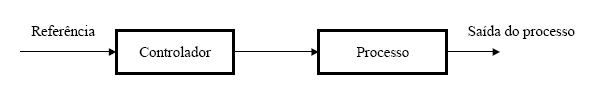
\includegraphics[width=\linewidth]{img/rf-malha_aberta.jpg}
				\caption{Sistema onde utiliza-se Malha Aberta. Sistemas que não possuem realimentação.}
				\label{fig:malha_aberta}
			\end{figure}

			Dessa forma, o processamento de dados é puramente absoluto, sem observar dados de processamento anteriores tendo assim uma visão unicamente momentânea.

			Um exemplo disso no caso aqui trabalho é o armazenamento dos valores de \textit{Pulse-Width Modulation} (PWM) do primeiro carro, e a execução direta desses valores num segundo carro ignorando o erro relativo que os motores geram entre si no ambiente testado. Essa prática não permite o controle de velocidade dos motores de corrente contínua utilizando apenas os valores de PWM tornando o controle do tipo Malha Aberta.


		\subsubsection{Malha Fechada}
			Já o sistema de controle em malha fechada, também é denotado de sistema de  controle  por  realimentação.

			A  saída $ y $ é  medida e comparada com   a   saída   desejada,   indicada   através   da referência $ r $,   para processamento  através  do  controlador  e  a  consequente  definição  da  ação  de controle $ u $, exibido em Figura \ref{fig:malha_fechada}.

			\begin{figure}[h]
				\centering
				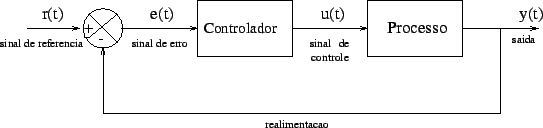
\includegraphics[width=\linewidth]{img/rf-malha_fechada.png}
				\caption{Sistema onde utiliza-se Malha Fechada. Sistemas onde existem um mecanismo de realimentação no controle de determinada ação.}
				\label{fig:malha_fechada}
			\end{figure}

			Neste trabalho é utilizado Malha Fechada. O sistema de realimentação utiliza como entrada, dados de processamentos anteriores criando assim uma proporcionalidade mais autêntica á situação a ser trabalhada. Ela será discutida ao decorrer do relatório.


	\subsection{Sistema Controlador Proporcional Usando Equação Diferencial Lineal de Primeira Ordem} \label{sec:eql1}
		Sistemas de controle é um sistema que possui o propósito de gerenciar o comportamento de outros dispositivos. Pode-se dizer que é uma interconexão de componentes conectados de maneira a comandar, controlar ou ajustar a si mesmo ou outro sistema obtendo uma precisão maior em seus procedimentos.

		A teoria de controladores proporcionais se baseiam em sistemas realimentados. Tais podem ser divididos em basicamente três partes sendo elas:

		\begin{itemize}
			\item Sistema a ser controlado;
			\item Controlador; e
			\item Realimentação.
		\end{itemize}

		O sistema a ser controlado é constituído por atuadores capazes de efetuar as ações necessárias. Os outros dois elementos têm como finalidade fazer com que o desempenho do sistema possua estabilidade e opere com certa precisão e agilidade, seguindo as especificações uma vez estabelecidas. Uma vez estabelecido como o sistema deverá ser desenvolvido, os controladores e sua realimentação serão item essencial para que o processo ocorra de forma estável. Tudo isso pode ser observado no diagrama exibido na Figura \ref{fig:estrutura_sistema_controle}.

		\begin{figure}[h]
			\centering
			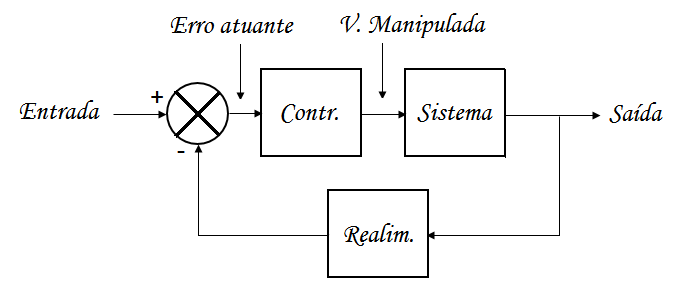
\includegraphics[width=\linewidth]{img/math-realimentacao.png}
			\caption{Estrutura de Sistema de Controle Geral Realimentado.}
			\label{fig:estrutura_sistema_controle}
		\end{figure}

		A realimentação é o ponto chave para a diferenciação de sistemas controladores comuns. Um sistema de controle realimentado compara, instantaneamente, o valor de saída anterior, com o valor de referência existente na entrada do sistema como os sensores. O resultado desta comparação é o centro de toda adaptabilidade estudada e é denominado erro atuante. Este é levado ao controlador, que produz o chamado sinal de controle, cuja função resume-se em reduzir o desvio entre a saída e o sinal desejado. Como o nome sugere, em um controlador proporcional a saída do mesmo, também conhecido como sinal de controle (ou ação de controle), é diretamente proporcional ao sinal de erro, ou seja, ao erro atuante.

		Sabendo-se em da proporcionalidade direta entre o sinal de controle e o sinal de erro, é possível afirmar que

		\begin{equation}
			a(t) \propto e(t)
		\end{equation}

		onde o controle é diretamente proporcional à seu erro.

		Entretanto, não é possível realizar operações matemáticas exatas com o sinal de proporção da fórmula. Para isso, deve-se admitir então uma constante de proporcionalidade entre as mesmas. Esta possui o nome de ganho proporcional e é representado pela variável $f$. Sendo assim

		\begin{equation}
			a(t) = f * e(t) \label{eq:formula_geral}
		\end{equation}

		e dessa forma, o sistema matemático mostrado na Equação \ref{eq:formula_geral} poderá ser representado pelo diagrama exibido na Figura \ref{fig:sistema_dominio_tempo}.

		\begin{figure}[h]
			\centering
			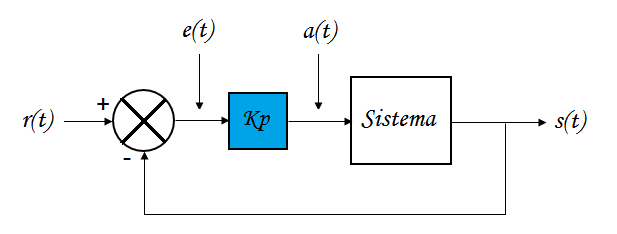
\includegraphics[width=\linewidth]{img/math-diagrama_geral.png}
			\caption{Sistema no Domínio do Tempo Geral.}
			\label{fig:sistema_dominio_tempo}
		\end{figure}

		Sendo assim, como fórmula final, temos

		\begin{equation}
			a(t) = f * (r(t) - s(t))
		\end{equation}

		onde $a(t)$ é a atuação, $e(t)$ representa o erro, $ r(t) $ é o valor de início de execução de controle e $ s(t) $ é saída do controle. Todos representando o valor no tempo $t$.


	\subsection{Velocidade Angular} \label{sec:velocidade_angular}
		A diferença gerada entre cada intervalo de tempo permite calcular a velocidade angular de cada motor como é exibido na Figura \ref{fig:angular_velocity}.

		\begin{figure}[h]
			\centering
			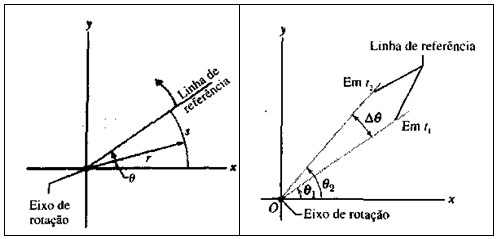
\includegraphics[width=0.65\linewidth]{img/math-angular_velocity.jpg}
			\caption{Ilustração do cálculo da velocidade angular.}
			\label{fig:angular_velocity}
		\end{figure}

		Para exemplificação, suponha que motor está em movimento de rotação. Em um dado instante $t_1$, encontra-se à um certo ângulo $\theta_1$ medido em relação à certo ponto. Após certo tempo, no instante $t_2$, encontra-se à um certo ângulo $\theta_2$ medido em relação ao mesmo ponto. Denomina-se velocidade angular média a taxa de variação temporal de tais ângulos. Ou seja,

		\begin{equation}
			\omega = \frac{\theta_2 - \theta_1}{t_2 - t_1} = \frac{\Delta \theta}{\Delta t},
			\begin{cases}
				\Delta \theta & \quad \text{é o deslocamento angular}\\
				\Delta t      & \quad \text{é a variação de tempo}\\
			\end{cases}
		\end{equation}

		sendo a velocidade angular instantânea é determinada quando o valor de $\Delta t$ tende a zero

		\begin{equation}
			w = \lim_{\Delta t \to 0} \frac{\Delta \theta}{\Delta t} = \frac{d \theta}{d t}
		\end{equation}

		lembrando que $ 2 \pi\ rad = 360\degree$.


\section{Elementos do Projeto} \label{sec:elem-teo}

	\subsection{Visão Geral da Especificação}
		Como já mencionado na Especificação (Seção \ref{sec:especificacao}), existirá dois robores e uma computação em nuvem.

		O trabalho consiste em replicar as ações de um carro $ \mathcal{A} $ repleto de sensores em um carro $ \mathcal{B} $ inexistindo os sensores de luz para detecção de faixa. Além disso, o processamento de dados e tomada de decisões será totalmente feita em nuvem, deixando os carros unicamente como plataformas de leitura de sensores e atuadores.

		Como é representado na Figura \ref{fig:diagrama}, o carro $ \mathcal{A} $ terá sensores e atuadores. Seus dados não serão processados nele em si, mas sim em um computador externo ao sistema atuador. Após a execução do trajeto, a \textit{cloud} teria dados suficientes, providos de vários sensores, para fazer o carro $ \mathcal{B} $ realizar o mesmo trajeto.

		Para que isso possa ser realizado, cada carro terá seus dispositivos e um componente Wi-Fi para envio e recebimento de dados sem fio à \textit{access points} e assim conexão com a \textit{cloud}.

		\begin{figure}[h]
			\centering
			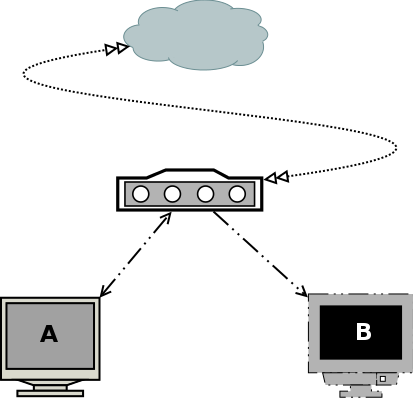
\includegraphics[width=0.5\linewidth]{img/diagrama_geral.png}
			\caption{Diagrama Geral Abstrato do Sistema.}
			\label{fig:diagrama}
		\end{figure}

		Deve-se atentar que os dois carros possuem características e propósitos diferentes e que todo o processamento é realizado na \textit{cloud} e não nos carros sendo estes somente para captação de dados e execução de tarefa com seus atuadores.

		Abaixo será descrito cada componente do sistema e algumas propriedades importantes.

	\subsection{Sensores do Carro $ \mathcal{A} $}
		O projeto do carro $ \mathcal{A} $ utilizou-se de vários tipos de sensores.

		Utilizar somente o sensor fototransistor seria suficiente para o projeto de seguido de linha, mas não para este em si que necessita de um item controlador. Sua função é unicamente para direcionar o carro informando o controle a situação para que ele não saia da linha completando o trajeto. Usando somente ele, é impossível que o carro saiba sua posição e seus movimentos para a reprodução no segundo carro.

		Para contornar este problema, necessita-se de do sensor de contador de giros da roda chamado \textit{Encoder}. Ele, junto com o fototransistor, serão mencionados nas Seções \ref{sec:fototransistor} e \ref{sec:movimentos}.


		\subsubsection{Sensor de Luz - Fototransistor} \label{sec:fototransistor}

			\paragraph{Tecnologia}
				Para o carro, será utilizado o sensor fototransistor. Em sua superfície, existirá um LED que fará a iluminação da área no qual refletirá sobre a superfície e chegará até o sensor fototransistor. Como o seguidor de linha move sobre dois tipos de superfície (branca e preta), é possível identificar quando ele sairá da direção correta. Essa ideia melhor visualizada com a Figura \ref{fig:ft}.

				\begin{figure}[h]
					\centering
					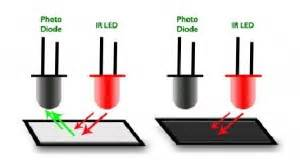
\includegraphics[width=0.45\linewidth]{img/elementos-fototransistor.jpg}
					\caption{Funcionamento do sensor Fototransistor.}
					\label{fig:ft}
				\end{figure}

			\paragraph{Propósito do Projeto}
				O projeto utilizará não somente dois sensores deste tipo mas uma série deles, posicionados logo à extremidade da faixa de direção como é exibido na Figura \ref{fig:dois_sensores}.

				\begin{figure}[h]
					\centering
					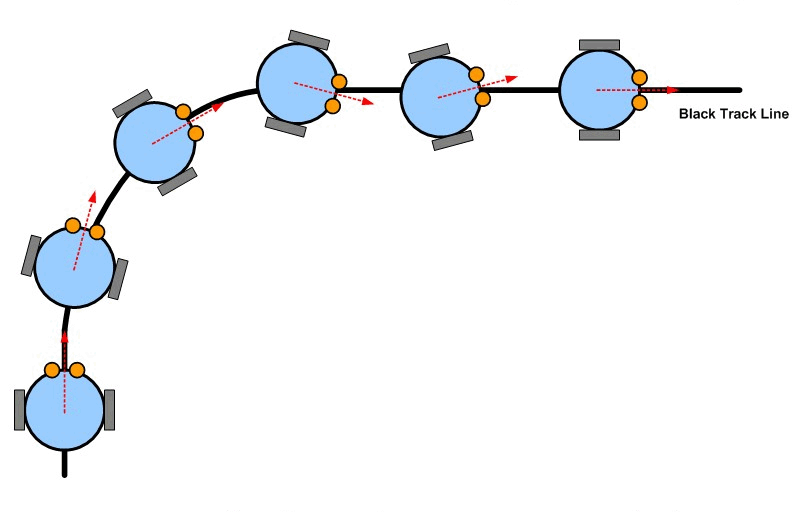
\includegraphics[width=0.9\linewidth]{img/elementos-line_tracking.png}
					\caption{Posição dos Sensores. Exemplo utilizando dois sensores.}
					\label{fig:dois_sensores}
				\end{figure}

				Utilizando uma série de sensores, cada sensor será responsável por avaliar se o carro saiu da linha original. Quanto mais à extremidade a faixa estiver em relação à série de sensores, maior será o erro dela e assim, a consequente uma correção mais rápida. Quanto maior a quantidade de arranjo de sensores melhor será a performance do carro pelo motivo que mais sensores representarão melhor o nível do erro. Por este motivo, será utilizado seis sensores, posicionando três em cada extremidade da faixa. Eles serão dispostos o mais próximo possível de seu adjacente pois a resolução de operação será melhor do que distâncias grandes como três centímetros ou mais. Um exemplo com 8 sensores é exibido na Figura \ref{fig:sensores_series}.

				\begin{figure}[h]
					\centering
					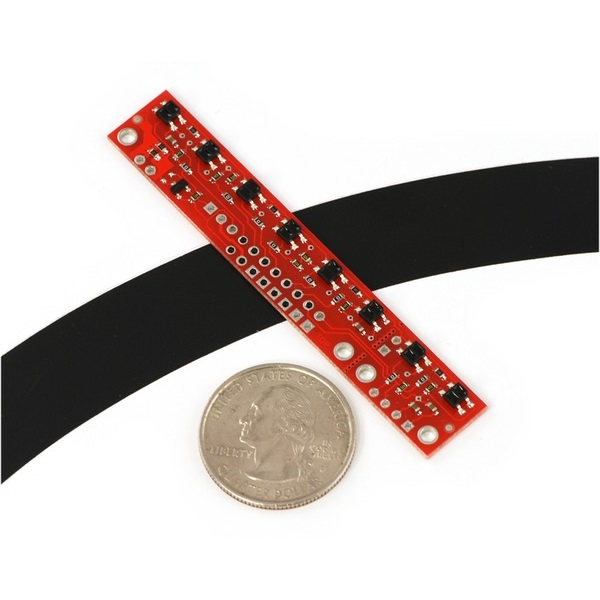
\includegraphics[width=0.7\linewidth]{img/elementos-sensores_series.jpg}
					\caption{Sensores posicionados em uma \textit{board} em série.}
					\label{fig:sensores_series}
				\end{figure}


		\subsubsection{Sensores de Movimento} \label{sec:movimentos}
			Como já descrito na Seção \ref{sec:fototransistor}, sensores fototransistores não conseguem realizar gravações de que detectam movimento. Para suprir essa necessidade utilizar-se-á um sensor que contará a quantidade de rotações que a roda fará.

			\paragraph{Codificador de Rotações} \label{sec:encoder}
				Um \textit{rotary encoder}, é um dispositivo eléctro-mecânico que converge a movimento do eixo para valores digitais/analógicos. O sensor utilizado foi do tipo incrementa/relativo no qual a saída do \textit{encoder} provê informações sobre o movimento do eixo no qual é possível obter informações de velocidade, distância e posição.

				Ele trabalha percebendo alteração de posição no qual deve ser analisado e processado por um componente externo a ele, que no caso deste trabalho é o próprio controlador.

				A Figura \ref{fig:encoder} exibe o mecanismo de leitura de movimento dos \textit{encoders} utilizados no trabalho.

				\begin{figure}[h]
					\centering
					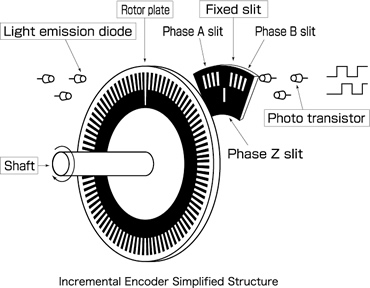
\includegraphics[width=0.6\linewidth]{img/elementos-encoder.jpg}
					\caption{Visão técnica sobre o funcionamento do \textit{encoder} para detecção de movimento.}
					\label{fig:encoder}
				\end{figure}

				Cada roda possui o formato $ 65mm $ por $ 30mm $ de largura. Uma rotação completa, segundo a fórmula $ P = d \pi $, mostra que o carro percorreu $ 204,2035224833 = 64 \pi $ mm, ou seja, cerca de $ 20,42 $ centímetros.

				O \textit{encoder} utilizado disponibilizado neste trabalho possui 20 furos. Isso permite um total máximo de 40 \textit{trick} ao analisar espaços vazados ou não. Sendo assim é possível calcular movimentos a cada $9\degree$ rodados, significando detecções de movimentos a cada $\frac{360}{20,42} = \frac{9}{x} \equiv 0,5105$ centímetros percorridos.

		\begin{comment}
		\subsubsection{Sensores de Movimento} \label{sec:movimentos}
			Como já descrito \ref{sec:fototransistor}, sensores fototransistores não conseguem realizar gravações de que detectam movimento. Para suprir essa necessidade utilizar-se-á de dois outro tipos de sensores que detectarão movimento. O acelerômetro e o giroscópio.


			\paragraph{Acelerômetro}
				Consegue capturar dados de duas à três dimensões (como mostra a Figura \ref{fig:accelerometer}) podendo reconhecer qualquer tipo de movimento do ambiente onde está instalado.

				\begin{figure}[h]
					\centering
					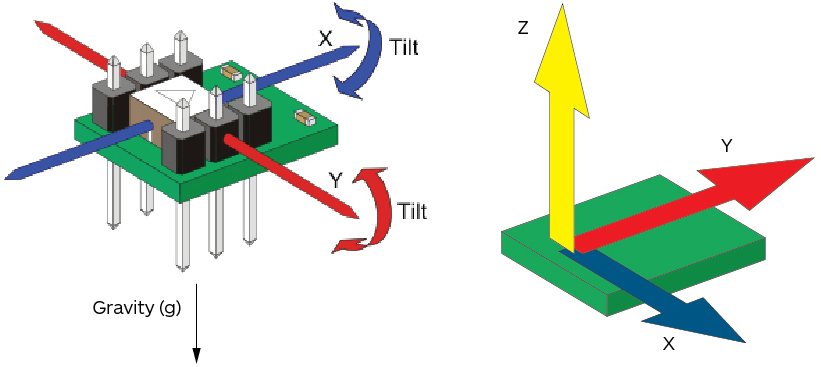
\includegraphics[width=0.9\linewidth]{img/elementos-accelerometer.jpg}
					\caption{Visão técnica sobre o funcionamento do acelerômetro.}
					\label{fig:accelerometer}
				\end{figure}

				O sensor acelerômetro será utilizado para captar dados de deslocamento do carro como aceleração e distância percorrida.

				Entretanto, velocidade e distância também não são suficientes para o projeto do carro como um todo, e por isso será mencionado o uso de giroscópio.


			\paragraph{Giroscópio}
				O giroscópio é um sensor que consegue captar a angulação de determinado objeto à ele instalado, mesmo depois de realizar movimentos.

				Assim, utilizando o aceleração e angulação, é possível registrar o trajeto que o carro realizou ao percorrer a trilha da faixa. Um exemplo da tecnologia utilizada hoje nos dispositivos embarcados é exibido na Figura \ref{fig:gyroscope}.

				\begin{figure}[h]
					\centering
					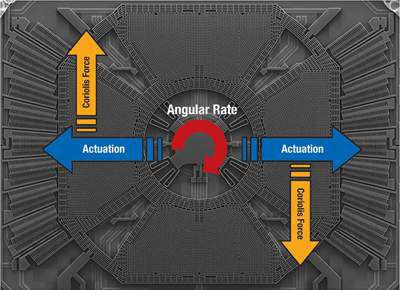
\includegraphics[width=0.6\linewidth]{img/elementos-gyroscope.jpg}
					\caption{Exemplo de giroscópio situado em telefones digitais modernos.}
					\label{fig:gyroscope}
				\end{figure}


			\paragraph{Resultado da Combinação desses Sensores}
				Assim, o sensor fototransistor realizará a leitura do trajeto a ser feito, o acelerômetro receberá a velocidade atual do carro e o giroscópio registrará a angulação do carro.

				Tudo isso processado permite a reprodução exata no carro $ \mathcal{B} $, mesmo sem utilizar nenhum sensor.
			\end{comment}


	\subsection{Atuadores}

		\subsubsection{Motores de Corrente-Contínua}
			Motores de corrente contínua baseiam-se no fluxo ordenado de elétrons sempre numa direção. São equipamentos que podem ser alimentados por tensões desde $1,2V$ até $24V$ e pode-se dizer de modo geral que é um equipamento que é capaz de converter energia elétrica em mecânica e vice-versa. 

			Falando de suas estruturas físicas, um motor de corrente contínua possui um conjunto de ímãs permanentes fixos, criando um campo magnético fixo enquanto o rotor é percorrido por uma corrente. Por meio de escovas e comutadores, a direção da corrente é alterada constantemente, fazendo com que o rotor gire continuamente. 
            %De forma analítica, se ímãs permanentes são usados para gerar o campo magnético, o torque de saída $T$ é proporcional ao fluxo magnético $\phi$ e à corrente nos enrolamentos do motor $i$.

			Possuem como vantagens a qualidade de serem bons para quaisquer tamanhos de robôs, engrenagens para redução de inércia, confiáveis, de baixa manutenção. Como pontos negativos, eles possuem baixa rigidez, necessidade de engrenagens para inúmeros projetos, folgas, custo, peso e necessidade de frenagem caso não alimentado.

			Diferente de motores de passo, no qual seu giro ocorre por meio de troca de suas angulações de forma sequencial, os motores de corrente contínua determinam sua velocidade de rotação com valores proporcionais à tensão no rotor. Como essa velocidade é totalmente relativa à tensão, é necessário componentes adicionais para determinar a velocidade de giro do motor. 
            
            As plataformas de prototipagem fornecem esses controles de tensão por meio de sinais PWM, descritos a seguir.

		\subsection{PWM}
			Os controles de potência PWM (\textit{Pulse Width Modulation}) são altamente indicados para aplicações em robótica pela possibilidade de se manter o torque mesmo em baixas velocidades. 

			Nos controles PWM o que se faz é variar a largura do pulso de uma tensão retangular aplicada à carga de modo obter-se um controle sobre a potência média aplicada, como é demonstrado na Figura \ref{fig:pwm}.

			\begin{figure}[h]
				\centering
				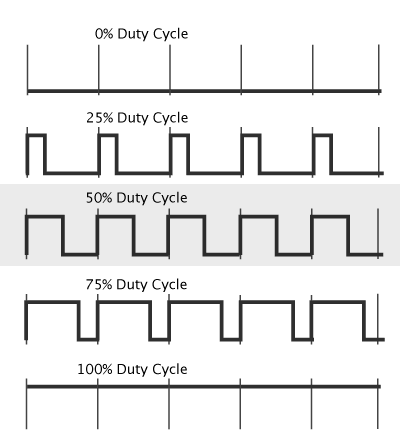
\includegraphics[width=0.5\linewidth]{img/math-pwm.png}
				\caption{Sinais PWM.}
				\label{fig:pwm}
			\end{figure}


		\subsubsection{Engrenagens de Redução}
			Motores elétricos giram em altas velocidades e quando necessita de torque elevado ou baixas rotações devem ser usados um conjunto de engrenagens de redução. 

			Naturalmente, isso aumenta o custo, o número de peças, a folga, a inércia do corpo rotativo, e assim por diante, mas também a resolução do sistema, já que com os trens de engrenagem é possível girar o elo de um pequeno ângulo como é demonstrado na Figura \ref{fig:reducao} um exemplo de redução.

			\begin{figure}[h]
				\centering
				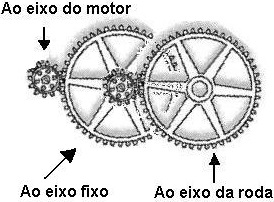
\includegraphics[width=0.5\linewidth]{img/math-reducao.jpg}
				\caption{Sistema simples de trens de engrenagens no qual gerará reduções.}
				\label{fig:reducao}
			\end{figure}

			Para um motor pequeno, esta taxa de redução permite uma multiplicação considerável de sua força, o que quer dizer que no eixo de redução obtém-se um torque considerável como produto final. Entretanto, o torque é obtido apenas no produto final de todo conjunto de trens de engrenagens. Isso significa que para o motor conseguir ter a torque/velocidade final requerida, ele deve enfrentar primeiro todo o processo inicial de movimentação das engrenagens que adicionam certa resistência ao conectar-se ao eixo do motor. Iniciado sua rotação, o motor terá a baixa rotação/torque requeridos.


		\subsubsection{Montagem}
			Como os motores obtidos para o trabalho possuem alta velocidade para a movimentação do carro, será utilizado além de caixa de reduções, sensores para captação de dados de velocidade, onde seus dados serão enviados para a \textit{cloud}, processados e recebidos novamente para assim realizar a atuação no carro. Isso exceto no caso do Carro \textit{B}, no qual não haverá processamento, mas sim somente sua atuação, sendo este somente um receptor escravo.

			Todos esses componentes serão acoplados à \textit{board} utilizando um \textit{motor shield} intermediário entre o microcontrolador e os motores. Tal \textit{motor shield} realizará o processo de interface de controle e energização dos motores criando assim um sistema estável. Seu nome é L293DD e possui suporte total para interface de pinos NodeMCU. Seu sistema de operação utiliza Ponte-H dupla e com isso é possível controlar até dois motores além de conectores para seleção de interface serial UART, SPI, e entrada analógica, além de conexões para habilitar as opções de \textit{Enable} e \textit{Reset} do microcontrolador. Ele pode ser visto por meio da Figura \ref{fig:eq-motor_shield}.

			\begin{figure}[h]
				\centering
				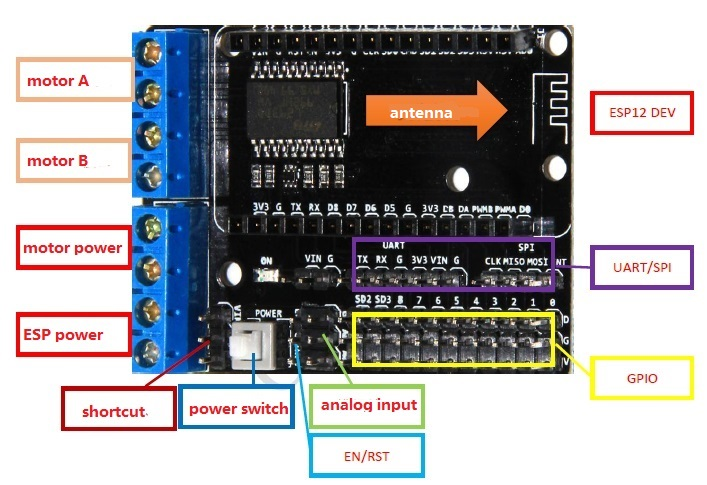
\includegraphics[width=0.9\linewidth]{img/elementos-motor_shield.jpg}
				\caption{Motor \textit{Shield} a ser Utilizado.}
				\label{fig:eq-motor_shield}
			\end{figure}

			No conjunto de componentes também é incluído duas rodas de borracha com $65mm$ e $30mm$ de largura.



		\begin{comment}
	\subsection{Visão Geral do Controle} \todo{a}
		O carro, ao andar pra frente, ficará numa velocidade\footnote{Velocidade monitorada pelo \textit{encoder} e o controlador.} máxima fixa. Quando algum de seus sensores perceber que o carro saiu da linha gerando uma interrupção, o procedimento de correção de direção será acionada para avaliar os dados dos sensores e assim verificar os passos a serem realizados nos atuadores para que o carro volte a operar normalmente na direção correta em cima da faixa.

		%Existem dois tipos de comportamentos em um seguidor de linha comumente conhecido. Eles serão descritos e explicados a seguir.


		\subsubsection{Comportamentos de um Sistema Sem Controle}
			Neste exemplo onde não possui-se realimentação no controle, mostrado na Figura \ref{fig:trajeto2}, é possível perceber que, carro fará seu trajeto com muita dificuldade. Seu meio de processamento baseia-se unicamente no ato parar totalmente o carro ao esbarrar na linha. Este tipo de controle funciona, mas não traz uma otimização aos movimentos realizados pelo carro, pois o carro não utiliza nenhum recurso de realimentação para realizar movimentos mais precisos.

			\begin{figure}[h]
				\centering
				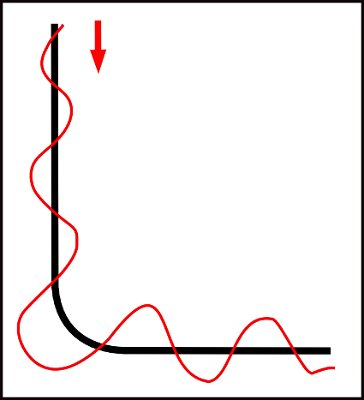
\includegraphics[width=0.5\linewidth]{img/elementos-trajeto2.jpg}
				\caption{Trajeto esperado de um seguidor de linha comum.}
				\label{fig:trajeto2}
			\end{figure}

			%O movimento oscilatório exibido na Figura \ref{fig:trajeto2} faz com que o carro gaste tempo em completar sua tarefa de percorrer a linha e também energia, item essencial para sistemas embarcados. 
			%Nesta situação relacionando à especificação do trabalho, o carro $ \mathcal{A} $ com seus movimentos oscilatório gerarão um mapa do trajeto complexo o suficiente para que o carro $ \mathcal{B} $ não consiga finalizar sua tarefa. Tais movimentos oscilatórios podem fazer o carro  $ \mathcal{B} $ se perder facilmente com o acúmulo de erros em cada movimento realizado.


		%\subsubsection{Comportamentos Sobre Controle Proporcional}
		%Utilizando um controle proporcional, o carro terá um fator de realimentação no qual passará a ter movimentos mais suaves e relativos às suas atividades e assim, seu trajeto poderá ser mais conciso quanto à linha do trajeto a ser executada. 
		%O resultado esperado é exibido na Figura \ref{fig:trajeto3}.

		\begin{figure}[h]
			\centering
			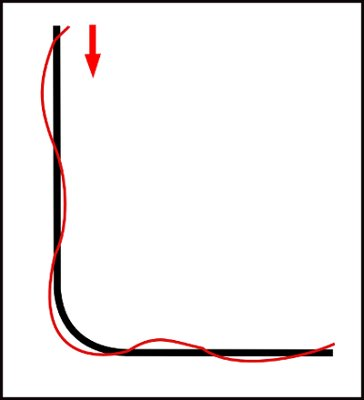
\includegraphics[width=0.5\linewidth]{img/elementos-trajeto3.jpg}
			\caption{Trajeto esperado de um seguidor de linha utilizando Controle Proporcional.}
			\label{fig:trajeto3}
		\end{figure}

		%Um fato importante a se atentar é que, para que o carro funcione como esperado, o algoritmo, seus parâmetros e os parâmetros da fórmula de controle proporcional devem estar devidamente calibrados para que o carro obtenha a melhor performance possível.

		%Este trajeto faz com que seus movimentos sejam mais suaves, estáveis, ágeis e eficientes em relação ao mostrado na Figura \ref{fig:trajeto2}, exibida anteriormente.
		\end{comment}

	\subsection{Microcontrolador}
		Microcontrolador utilizado para este trabalho é o NodeMCU. É um plataforma IoT\footnote{\textit{Internet of Things}, ou seja, internet das coisas.} \textit{open-source}.

		Como esperado de um microcontrolador para IoT o sistema possui integrado um componente de comunicação Wi-Fi para troca de dados. Utiliza linguagem de \textit{script} Lua desenvolvida por brasileiros ou IDE e linguagem Arduino.

		Suas especificações são uma CPU ESP8266 possuindo 128 KB de memória, 4 MB de armazenamento e suporta o sistema operacional chamado XTOS. Permite comunicação pelo Wi-Fi e USB onde também é energizada. Possui um total de 10 pinos de entrada e saída de propósito geral (GPIO) onde suportam funções como PWM, comunicação I$ ^2 $C e 1-wire. Além da antena Wi-Fi, possui também um conversor USB-TTL para comunicação serial.

		A Figura \ref{fig:eq-nodemcu} exibe um esquemático de seu protótipo.

		\begin{figure}[h]
			\centering
			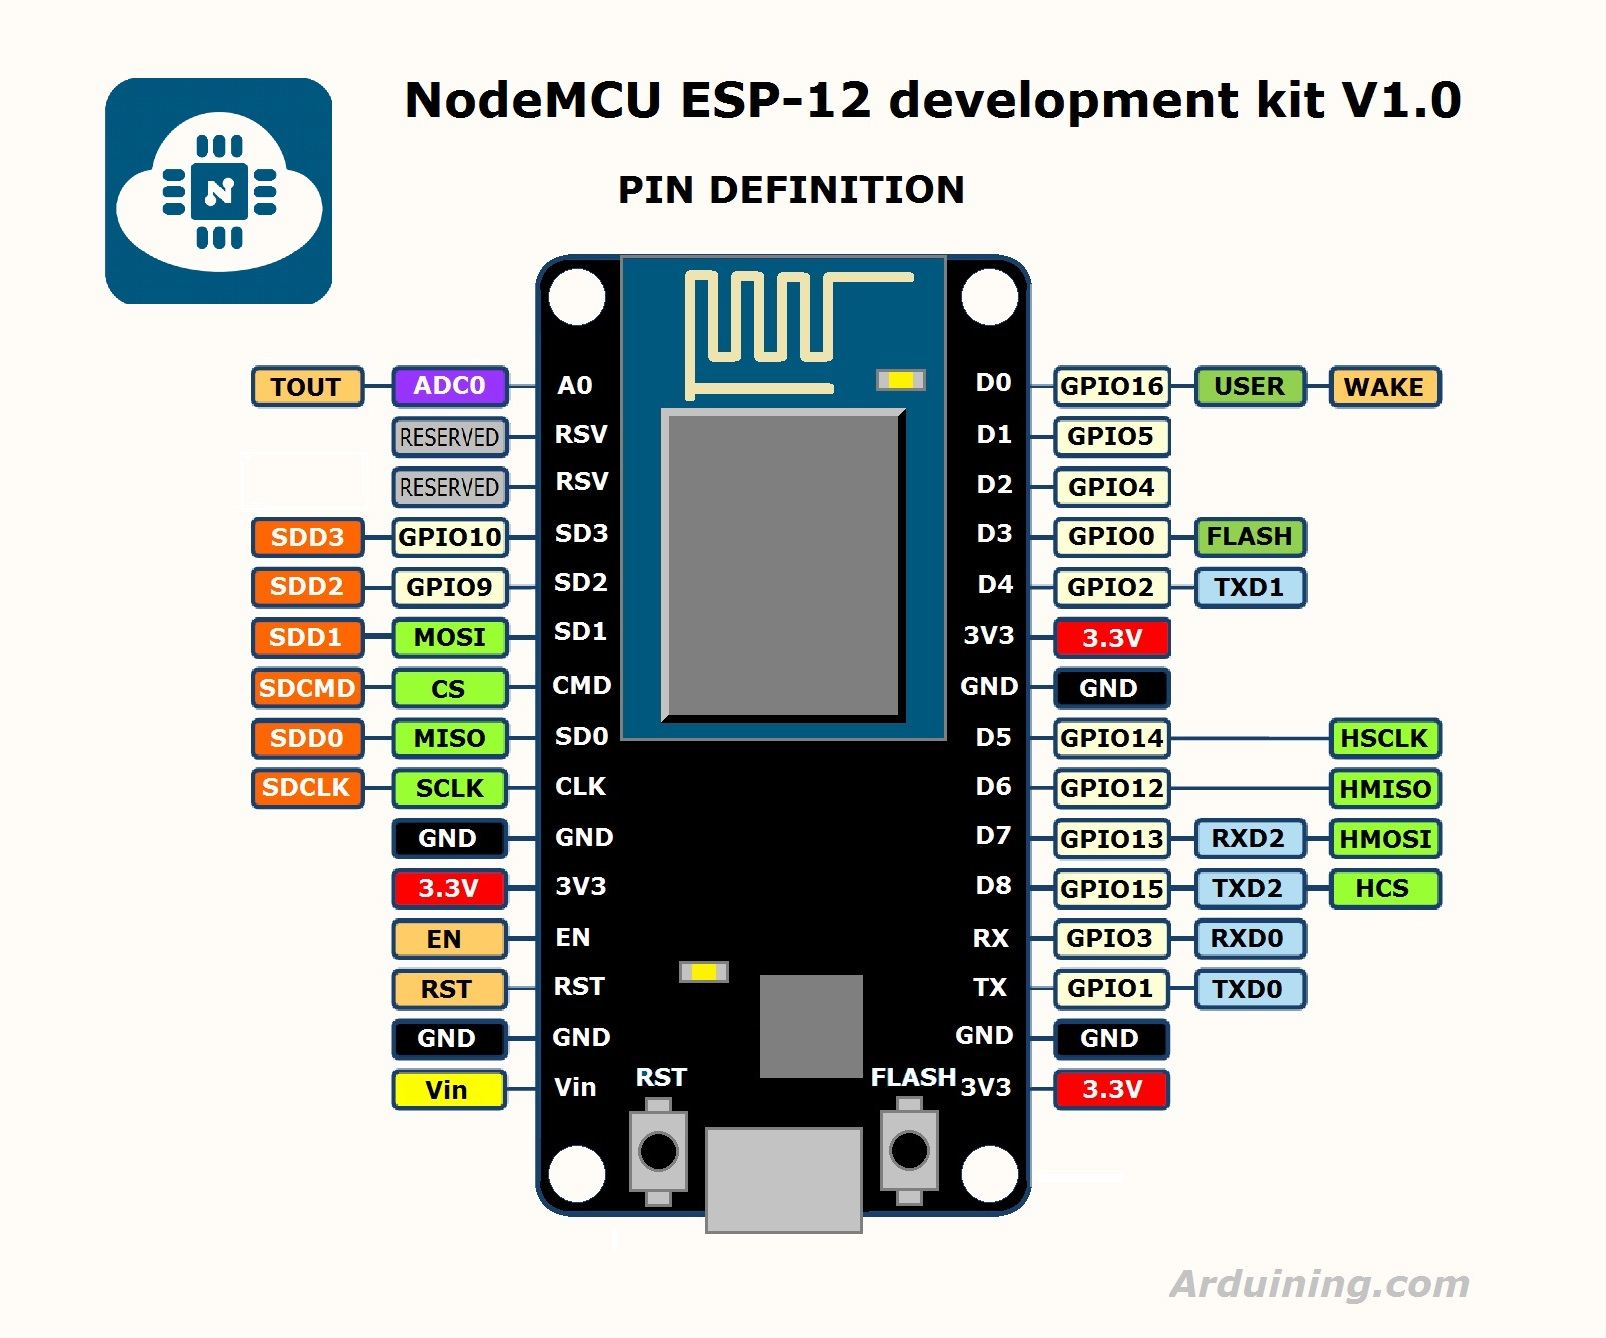
\includegraphics[width=0.99\linewidth]{img/elementos-nodemcu.jpg}
			\caption{O Microcontrolador NodeMCU e seus Componentes e I/O.}
			\label{fig:eq-nodemcu}
		\end{figure}

		Sua programação pode ser feita por diversas maneiras. As duas principais são utilizando um terminal serial para envio de comandos diretamente à placa usando a porta USB do controlador.

		Como ela possui placa de comunicação Wi-Fi e um controlador poderoso, é possível também transformá-la num \textit{Web Service} para que realize toda a comunicação sem fio.


	\subsection{Alimentação}

		Os motores devem ter como entrada $6V$ e possui velocidade média de $90\pm10rpm$ com corrente de 250 mA sem carga. Sua corrente de partida pode chegar a $1A$.

		Utilizando um \textit{jump}, é possível criar um curto de tal forma que os motores e o NodeMCU poderiam ser energizados por tal, permitindo total controle e a utilização de nenhum fio para alimentação do sistema.

		Sua energização será realizada por meio de fonte externa utilizando dois \textit{pack} de 4 pilhas em série.

		Utilizar uma fonte por meio da interface USB diretamente no microcontrolador não seria suficiente para energizar todos os atuadores e sensores do sistema. Dessa forma, a fonte externa alimentará os atuadores e o microcontrolador e este alimentará todos os sensores nele contido.


	\subsection{Nuvem}
		Como os processadores não podem realizar processamento seguindo a especificação, utilizou-se de um servidor construído em Python para a comunicação e processamento de ambos os carros. Utilizar este tipo de sistema traz várias vantagens com redução de gasto energia nos carros e centralização de processamento e \textit{backup} de informações em local seguro além da transparência do sistema de controle. Também permite que as configurações de execução do carro sejam feitas totalmente via servidor, já que este enviará controles aos carros.

		Entretanto, latências altas em comunicações ou pacotes de informações corrompidas e interferências de ambiente podem tornar o sistema inconsistente ou até mesmo comprometido para seu propósito.


\section{Modelamento Matemático} \label{sec:math}

	\begin{comment}
	
	\subsection{Teoria da Equação Diferencial Linear}
		Equações Diferenciais Lineares são equações que suas soluções podem ser somadas a fim de produzir uma nova solução.

		É considerada linear quando satisfaz as características de que cada coeficiente a $a_{n}$ e o termo de não-homogeneidade só dependem da variável independente, no caso $x$; e a variável dependente, no caso $y$, e suas derivadas são de primeiro grau. Assim, ela deve representar a seguinte forma

		\begin{equation}
		f(x) = a_{n}(x)\frac{d^{n}y}{dx^{n}} + a_{n-1}(x)\frac{d^{n-1}y}{dx^{n-1}} + \cdots +  a_{1}(x)\frac{dy}{dx} + a_0(x)y
		\end{equation}

		No uso para problemas que utilizam Controle Proporcional descrito no Seção \ref{sec:controle_proporcional}, basta desligar todas as derivadas e integrais da equação obtendo

		\begin{equation}
		f(x) = a_{n}(x) + a_{n-1}(x) + \cdots +  a_{1}(x) + a_0(x)y
		\end{equation}
	\end{comment}


	\subsection{Definições}
		%https://syclops.wordpress.com/2011/08/06/part-2-line-following-robot-code-guideline-arduino-using-pid/
		Para iniciar a discussão sobre sistema de controle proporcional, primeiramente será definido os termos utilizados. 

		\begin{description}
			\item[\textit{Alvo:}] É a posição que desejamos que o carro esteja em relação à faixa, ou seja, centralizado respeitando a devida linha.

			\item[\textit{Erro:}] Diferença entre a posição atual e o \textit{Alvo}. Pode ser qualquer valor no conjunto dos ${\rm I\!R}$.

			\item[\textit{Proporção:}] Fator que determinará quão distante o carro está da linha. Por exemplo são as proporções: `\textit{para a esquerda}',  `\textit{para a direita}', `\textit{para a extrema esquerda}', `\textit{pouco para a direita}', etc. É representado pela constante de variação $ K_p $.

			\begin{comment}
				\item[\textit{Integral:}] Proporciona o erro acumulado sobre o tempo corrido. Isso significa que este irá informar se o carro vem estando na linha nos últimos momentos ou não. Representada pela constante de variação $ K_i $.

				\item[\textit{Derivada:}] Taxa no qual exibe a oscilação do carro sobre a linha, representada pela constante de variação $ K_d $.
			\end{comment}

		\end{description}

		%Ambos \textit{Integral} e \textit{Derivada} utilizam o valor \textit{Proporção}.

		O procedimento de execução é baseado no seguinte pseudocódigo:
		\begin{enumerate} \it
			\item Realiza o cálculo inicial da posição atual.

			\item Calcula o erro baseado na posição atual.

			\item Ele então comandará os motores para fazer uma girada:
			\begin{itemize}
				\item \underline{Brusca} caso o erro for grande; ou
				\item \underline{Leve} caso o erro for pequeno.
			\end{itemize}
			Assim, basicamente, a magnitude do giro tomado é proporcional ao \textit{erro}.

			\item Repete os passos até completar o objetivo proposto.
		\end{enumerate}

		Com esses passos, saímos de um controle simples para um Controle Proporcional mais eficaz.

		\begin{comment}

			Mesmo se depois desses passos o valor de \textit{erro} não decrementar ou decrementar de forma bem lenta, ao realizar o passo 4, o controlador fará uma nova avaliação incrementando a magnitude de conserto de posição realizando novamente de forma mais brusca a tentativa de posicionar o carro novamente à posição centralizada. Esse processo só é possível por causa do Controle Integral. O efeito de redução de oscilação por tempo é trabalho pelo Controle Derivativo.

			O Controlador Proporcional Integral-Derivativo, também chamado de Controlador PID, é uma metodologia de cálculo de controle de processo que une várias outras menores. Utiliza de teorias como as Ações Derivativa (Controle PD), Integral (Controle PI) e Proporcional (Controle P).

			Estes quatro modos de controle, incluindo PID, são também designados de ações de controle, cada uma delas reagindo de forma distinta ao erro presente nos sistemas. O controle:

			\begin{itemize}
				\item Proporcional: ajusta a variável de controle de forma proporcional ao erro;
				\item Integral: ajusta a variável de controle baseando-se no tempo em que o erro acontece;
				\item Derivativo: ajusta a variável de controle tendo como base a taxa de variação do erro; e
				\item A combinação destes tipos de controle forma o controlador PID.
			\end{itemize}

		\end{comment}

		São amplamente utilizados em situações que se baseiam em controladores eletrônicos chamados ``\textit{single-loop}''.

		Abaixo é descrito a formulação matemática do conceito de controlador proporcional

	\subsubsection{Teoria de Controle Proporcional (P)} \label{sec:P}
		Produz um sinal de saída que é proporcional ao parâmetro do erro

		\begin{equation}
		P_{t} = P_{t-1} \times K_{p}\,{e(t)} \label{math:p}
		\end{equation}

		onde:

		\begin{description}
        	\item[$ P_t $\textit{:}] Relação de atuação no tempo $t$;
			\item[$ t $\textit{:}] Leitura dos sensores no tempo $t$;
			\item[$ e(t) $\textit{:}] Erro relativo ao tempo $ t $;
			\item[$ K_p $\textit{:}] Constante relativa à proporção, chamado de ganho proporcional.
		\end{description}

		%Esse método possui a propriedade de eliminar as oscilações do sinal de saída. 
        %Para tal, o sistema permanece sempre ligado e o sinal de saída é diferente de zero.
        Dessa forma, sobre a Equação \ref{math:p}, a proporção de erro é dada pela constante $K_p$, o erro pela função $ e(t) $ e o alvo é o valor de $ P_{t} $ no qual será o valor que o controle obteve a fim de obter a melhor performance em relação ao alvo imposto.

	\begin{comment}
		\subsection{Funcionamento Teórico-Procedural}
			Aqui será descrito uma representação de como será a implementação de toda a teoria descrita neste trabalho. Assim, de forma geral, teremos o seguinte algoritmo implementado para tratamento dos valores obtidos dos sensores e ajuste da rotações dos motores.

			\begin{algorithm}[h]
				\caption{Controle Proporcional de Correção de Angulação}\label{euclid}
				\begin{algorithmic}[1]
					%\Procedure{proportional\_control}{$ position, set\_point, \Delta, \int, last\_\Delta, y', \Phi $}
					\Procedure{proportional\_control}{$ position, set\_point, \Delta, last\_\Delta, \Phi $}

					\State $ \Delta \gets position - set\_point $
					%\State $ \int \gets \int + \Delta $
					%\State $ y' \gets \Delta - last\_\Delta $
					\State $ \Phi \gets \Delta * K_p $
					%\State $ \Phi \gets \Delta * K_p + \int * K_i + y' * K_d $
					\EndProcedure
				\end{algorithmic}
			\end{algorithm}

			onde:

			\begin{description}
				\item[\textit{position:}] Posição atual do carro.

				\item[\textit{set\_point:}] Ponto central onde encontra-se a faixa.

				\item[$ \Delta $\textit{:}] Representa o erro proporcional da posição atual contra o ponto central da faixa.
do
				%\item[$ \int $\textit{:}] Representa o acúmulo de erro atual.

				\item[$ last\_\Delta $\textit{:}] Representa o erro proporcional da posição da iteração passada.

				%\item[$ y' $\textit{:}] Retêm a diferença entre os erros atual e da iteração anterior.

				\item[$ \Phi $\textit{:}] Correção a ser realizada nesta iteração.
			\end{description}

			Como é de se esperar, a correção proporcional $ \Phi $ será aplicada à velocidade motor para conserto de posição do carro.
	\end{comment}
\part{Desenvolvimento} \label{sec:parte2}

Nesta parte do documento será descrito como cada carro e nuvem foram construídos (Seção \ref{sec:construcao}), os obstáculos encontrados no desenvolvimento e utilização dos equipamentos (Seção \ref{sec:obstaculos}) e o modelo de controle construído (Seção \ref{sec:recorrencia}).

\section{Construção e Uso de Serviços e Equipamentos} \label{sec:construcao}

	\subsection{Carro Robô $ \mathcal{A} $}
		A construção do carro $ \mathcal{A} $ se baseou-se num sistema de sensores e atuadores que realiza leituras do ambiente por meio de interrupções de sistema e o envio desses dados para a nuvem. Tais dados são processados e retornados para o carro para assim ser realizado a atuação apropriada à situação segundo os cálculos do controle proporcional situado na nuvem.

		Ele possui dois sensores fototransistores na sua dianteira (Figura \ref{fig:robot_foto} na Seção Anexo) para detectar as faixas que orientam o carro e dois sensores encodificadores de rotação (Figura \ref{fig:robot_encoder} na Seção Anexo) para controle de velocidade/rotações.

		Além desses sensores, o carro é composto pois dois motores de corrente-contínua, dois \textit{pack} de pilhas e um NodeMCU junto com seu \textit{motor shield} e \textit{protoboard} para confecção do circuito elétrico, como mostrado na Figura \ref{fig:robot} na Seção Anexo.  
        

		%\subsubsection{Programação}
			O carro não possui nenhum tipo de processamento importante, sendo seu propósito único de leitura de sensores e atuação implicando numa programação simples de conexão com a nuvem, leitura, tratamento e envio dos dados e por fim sua atuação.

			A leitura do \textit{encoder} é feito por interrupção sistêmica no qual, a cada \textit{trick} alterado, o sensor realiza uma interrupção para incrementar o valor do grau de rotação naquele intervalo de tempo $t$. Tais detalhes serão explicados na respectiva seção da descrição do controle na nuvem, na Seção {sec:nuvem}.

			A detecção de faixa é feita por meio de interrupção de sistema gerando um procedimento de emergência de envio de dados para a nuvem a fim de obter resposta mais apropriada para a situação.


	\subsection{Nuvem} \label{sec:nuvem}

		O servidor foi desenvolvido utilizando linguagem de programação Python versão 2.7 que possui todos os artefatos necessários para a construção e utilização de uma aplicação com \textit{socket} para comunicação com aplicações externas.

		A nuvem recebe os dados lidos pelos sensores do carro a cada instante de tempo, definido como $30$ milissegundos, processa-os e responde o carro com os devidos comandos que ele deverá realizar sobre a situação imposta. Essa estratégia de arquitetura faz com que o processamento realizado seja inteiramente pela nuvem sendo a configuração de velocidade e de controle proporcional de execução do carro na pista sejam todas definidas via nuvem.

		%O teste de controle proporcional descrito na Análise Teórica do trabalho baseou-se na situação de que, caso encontre a faixa em algum lado do carro, a respectiva roda teria sua velocidade reduzida a ponto de que o carro possua a velocidade angular (Seção \ref{sec:velocidade_angular}) correta em cada roda para realizar a curva. Entretanto, os motores necessários não possuíam torque suficiente para o carro construído, impedindo este de realizar as movimentações necessárias como descrito na Seção \ref{sec:problema_motor}.
		
		%De forma a contornar este problema, construiu-se outra estratégia de controle proporcional que respeitasse o tempo de atuação que motor necessita para o funcionamento prático. 
        O algoritmo necessita de duas funções especiais para concluir seus cálculos sendo elas o Cálculo Proporcional (Algoritmo \ref{alg:control}) e o Cálculo de Rotação (Algoritmo \ref{alg:spin}). O primeiro algoritmo utiliza do controle P para gerar um valor de erro em relação à posição perfeita. Dado a posição atual $\Delta \Phi$ e a referência esperada $reference$, calcula-se a proporção de erro. Caso a referência seja o propósito de parar o motor, o erro 
        %será multiplicado pelo valor constante $10$ que 
        gerará um erro negativo o suficiente para solicitar a parada total do motor requerido. Obtido o erro proporcional, é feito o cálculo de velocidade do motor a fim de que tenha controle fechado sobre sua atuação. $erro = 0$ indica que o motor está na velocidade ideal. Valores positivos indicam que a potência do motor dever aumentada a fim de aproximar do requerido e negativo possui a ideia de decremento.

		\begin{algorithm}[H]
			\caption{Cálculo da proporção do erro em relação à posição referência.} \label{alg:control}
			\begin{algorithmic}[1]
				\Function{proprortion}{$\Delta \Phi, reference$}
					\State $position \gets \Delta \Phi;$
					\State $perfect\_position \gets reference; $
					\State $proportion \gets perfect\_position - position;$
					\State $error\_value \gets proportion * K_p;$
					\State \Return $error\_value;$
				\EndFunction
			\end{algorithmic}
		\end{algorithm}

		\begin{algorithm}[H]
			\caption{Cálculo da proporção de rotação dos motores sobre controle de malha fechada.} \label{alg:spin}
			\begin{algorithmic}[1]
				\Function{motors\_spin}{$\Phi, error, \Lambda$}
					\If {$\Lambda = NOT\_VISIBLE$}
							\State $rotation \gets (error * \Call{abs}{max\_rotation\_motor - rotation}) / 100$;
						\Else
							\State $rotation \gets - max\_rotation\_motor$;
					\EndIf
					
					\If {$rotation > MAX$}       \Comment{Verify if PWM value is in correct interval}
							\State $rotation \gets MAX$;
						\ElsIf {$rotation < MIN$}
							\State $rotation \gets MIN$;
					\EndIf

					\State \Return $rotation$;
				\EndFunction
			\end{algorithmic}
		\end{algorithm}

		Conhecido as funções básicas, é possível descrever o funcionamento do algoritmo de controle (Algoritmo \ref{alg:nuvem}). Ele receberá por parâmetro os valores de tempo, visualização de faixa do lado esquerdo e direito respectivamente, e somatório de \textit{tricks} de cada lado do carro, sendo respectivamente $ t, \lambda_l, \lambda_r, \phi_l, \phi_r $ suas variáveis. Cada procedimento descrito no algoritmo deverá ser processado para cada motor separadamente.

		O primeiro passo é o cálculo do deslocamento de cada motor no intervalo de tempo. Com o deslocamento, têm-se todos os dados de distância percorrido pelo carro. Verificando se o carro encontra-se sobre uma faixa, verifica-se seu erro proporcional. Caso o carro esteja sobre a faixa, o respectivo motor deverá parar enquanto o outro continua sua velocidade anteriormente estipulada. A partir do momento que sai da visualização de faixa, o controle proporcional inicia-se novamente para calcular a potência requerida ao motor para conseguir inércia suficiente para deslocar e chegar à velocidade angular requerida que é dada por $reference$.

		Tendo o erro referencial, calcula-se o valor de PWM pela função $motors\_spin$ e todos os dados relevantes da execução são salvos fisicamente em arquivo físico. Ao final, os novos valores de potência são enviados aos motores para que seja realizada a sua atuação e em seguida uma nova leitura dos sensores.

		\begin{algorithm}[H]
			\caption{Controle Proporcional em Nuvem.} \label{alg:nuvem}
			\begin{algorithmic}[1]
				\Procedure{proportional\_control}{$ t, \lambda_l, \lambda_r, \phi_l, \phi_r $}
					\State $\Delta \Phi \gets \Phi_{i} - \Phi_{i-1};$      \Comment{Angular displacement}

					\If {$\Lambda$}
							\State $error \gets $\Call{proportion}{$\Delta \Phi, reference$};
						\Else
							\State $error \gets $\Call{proportion}{$\Delta \Phi, 0$};
					\EndIf

					\State \Call{motors\_spin}{$\Phi, error, \Lambda$};
					\State \Call{save\_datas}{$t, rotation, \Phi$};
					\State \Call{send\_datas}{$rotation$};
				\EndProcedure
			\end{algorithmic}
		\end{algorithm}

		sendo:

		\begin{description}
			\item [$t$:] Instante de tempo da leitura dos sensores;
			\item [$\lambda$:] Leitura do respectivo sensor fototransistor indicando existência visual de faixa de cada lado do carro. Sendo $\Lambda$ representando operações em cada lado (esquero e direito), separadamente;
			\item [$\phi$:] Leitura dos \textit{tricks} de cada motor. Com $\Phi$ representando operações em cada lado (esquero e direito), separadamente.
		\end{description}

	\subsection{Carro Robô $ \mathcal{B} $}
		O carro robô $ \mathcal{B} $ é equipado com os mesmo equipamentos, com exceção do sensores fototransistores. Sua única função é se conectar com a nuvem mostrando sua identificação como carro com etiqueta $ \mathcal{B} $, receber o mapa do trajeto gerado pelo $ \mathcal{A} $ e executá-lo de forma a tentar reproduzir o trajeto.

		%\subsubsection{Programação}
			%Primeiramente utilizou-se da técnica mais simples que baseia-se na única tarefa de reproduzir os valores de PWM obtidos pelo carro $ \mathcal{A} $. Mas como essa abordagem de controle é do tipo de malha aberta, o carro ficaroa totalmente desgovernado, já que os valores não representarão de fato os movimentos realizados pelo primeiro utilizando este método.

			%Utilizou-se das leitura dos \textit{encoders} para auxiliar no controle de velocidade do carro a fim de criar um intervalo de confiança mais próximo de reprodução do carro $ \mathcal{A} $. 



\section{Análise dos Componentes e Obstáculos} \label{sec:obstaculos}
	Realizado a montagem dos componentes no carro, foi realizado testes com cada componente a fim de verificar a usabilidade de cada um e suas características físicas de funcionamento. Sendo assim, achou-se necessário descrever previamente os obstáculos obtidos com cada componente a serem considerados na construção controle proporcional do carro.

	\subsection{Atuadores e suas Caixas de Reduções} \label{sec:problema_motor}
		% Ele não conseguir para no tempo certo
        \subsubsection{Tempo de Atuação}
			Após realizados alguns testes com os motores, percebeu-se que eles possuem um pequeno atraso de resposta de resposta aos comandos. 
            
            Isso foi comprovado no teste de ação do carro ao perceber a presença de uma faixa. Quando o carro se depara com ela, indicando que deveria iniciar o processo de curva, as ações de alteração de velocidade ou mesmo de parada do motor não aconteciam num intervalo de tempo necessário para que o carro consiga de fato continuar dentro de sua trajetória. 

			A primeira hipótese considerada foi a latência gerada pela comunicação sem-fio na arquitetura distribuída. Entretanto, realizou-se novos testes com o sistema de controle situado totalmente no processador local do carro e o problema continuou persistindo, refutando a ideia da latência.

		\begin{comment}
		% torque suficiente para baixas rotações}
		% peso do carrinho?}
		\subsubsection{\todo{peso} da Estrutura contra Torque dos Motores}
			Além do problema do atraso do tempo de atuação, percebeu-se que o carro possui um \todo{peso} elevado em comparação à força de torque inicial que os motores acoplados a ele possuem, criando assim uma resistência maior para partida dos motores. 
			Em outras palavras, isso implica que o motor não possui torque suficiente para movimentar o carro em baixas rotações, necessitando de um valor alto de corrente para dar o torque inicial. 
			Como o carro é relativamente pesado para o motor, automaticamente a intensidade de corrente de partida aumenta para suprir a necessidade de movimentação, mas tal atuação não tem resultados positivos. 
			Motores de corrente de contínua não possui um controle de rotação e isso gera pulsos descontrolados no carro no qual o controle não consegue gerenciar bem os movimentos do carro criando assim uma trajetória complexa já pro carro $ \mathcal{A} $, aumentando ainda mais a dificuldade de reprodução do carro $ \mathcal{B} $.

			%Nas experiências com os motores, quando o carro conseguia vencer a inércia, a potência acionada ao motor era tamanha que o carro perdia o controle da velocidade acelerando o carro mais que o desejado tornando o mapa gerado pela aprendizagem mais caótico que o o esperado pelo projeto. Isso também é causado pela falta de força suficiente para mover o carro deste porte.

		\end{comment}
        
		%encoder
		\subsubsection{Controle de Velocidade Utilizando Encoder} \label{sec:problema_encoder}
        	Mesmo utilizando o \textit{encoder} para realizar o controle de velocidade, com base nos cálculos da Seção \ref{sec:encoder}, só é possível detectar movimento após $0,5105$ centímetros percorridos o que implica que, para o cálculo de velocidade do carro com mais precisão, ele precisaria andar numa velocidade maior para que obtivesse mais \textit{tricks} por intervalo de tempo.

			Isso pois, como os intervalos de tempo para cálculo e envio à nuvem são pequenos ($ 30 ms $), o cálculo da velocidade é dificultado pois taxa de \textit{tricks} por intervalo de tempo é pequena, cerca de 1 à 2, por tempo, impedindo de um controle de velocidade mais preciso.


		\subsubsection{Partida e Aceleração dos Motores}
			Nos teste com os motores e suas respectivas caixas, para que o carro conseguiesse vencer a inércia inicial, deveria injetar uma potência alta nos motores que o carro perdia o controle de direção por causa de sua brusca aceleração. Entretanto, a potência é alta o suficiente para desorientar o carro na sua aceleração.%Além do descontrole, foi percebido que o carro necessitava de altos valores de tensão para que conseguisse iniciar as rotações.

			O problema do descontrole gerado pela aceleração é que ao vencer sua inércia e iniciar a sua aceleração, o controle possui um certo atraso para detectar o início do movimento e gerenciar, logo em seguida, a velocidade requerida segundo a aceleração atual. Como mencionado em \ref{sec:problema_encoder}, o encoder não possui uma precisão fina sobre velocidade em taxas de tempo pequenas. Dessa forma, nessas acelerações o carro perde o controle ou excede a distância segura a ser percorrida.

		% dois packs de pilhas pesaram o motor}
		%\subsubsection{Uso de dois \textit{packs} de pilha}
			A relação de atuação e corrente dos motores seriam resolvidos ao adicionar mais corrente aos motores adicionando mais \textit{pack} de pilhas em paralela ao primeiro, por exemplo. Entretanto, realizou-se testes com \textit{pack} adicional para fornecer maior alimentação mas não obteve melhores resultados nos atuadores.

			Tanto com um e dois \textit{packs} de pilha, houve momentos que o controle colocou potência máxima nos motores com os dois \textit{packs} de pilhas acoplados ao carro e mesmo assim os motores não possuíam torque suficiente para dar a partida no carro, aumentando ainda mais a questão sobre o nível da resistência dos trens de engrenagens das caixas de reduções sobre a sua partida inicial.

		\begin{comment}
			% falar sobre a corrente de cada motor}
			Para confirmar todas essas hipóteses de que os motores não possuíam torque suficiente para move-lo, realizou-se testes de corrente em cada motor verificando se as pilhas foram devidamente suficientes para o sistema de motores. Com um multímetro, analisou-se os dois motores separados e em conjunto com um e dois \textit{packs} de pilhas, observando suas alimentações. Os resultados são exibidos na Tabela \ref{tab:valor_corrente} com os motores exercendo em potência máxima.

			\begin{table}[h]
				\caption{Tabela contendo os respectivos valores de intensidade de correntes para cada tipo de situação.}
			    \begin{tabular}{l|l|l|l}
			    \hline
			    ~                            & \textbf{I. de Partida} & \textbf{I. Nominal} & \textbf{I. Nominal com Atrito} \\ \hline
			    \textbf{1 Pack e 1 Motor}    & ~                      & 160                 & --        \\ \hline
			    \textbf{1 Pack e 2 Motores}  & ~                      & 250                 & 520       \\ \hline
			    \textbf{2 Packs e 1 Motor}   & ~                      & 160                 & --        \\ \hline
			    \textbf{2 Packs e 2 Motores} & ~                      & 255                 & 520       \\ \hline
			    \end{tabular}
			    \label{tab:valor_corrente}
			\end{table}

			Com tais valores é possível perceber que os motores não possuem torque suficiente para movimentação de um carro do porte (\todo{peso} de todos os equipamentos) no qual foi montado o trabalho. Como descrito, mesmo adicionando mais corrente ao circuito de motores, o \todo{peso} adicionado pelo novo \textit{pack} de pilha criou um \textit{trade-off} entre aumento de energia e de seu \todo{peso} para deslocamento. 

			Para contornar o problema do motor fraco, implementou-se um controle que, sempre que encontra uma faixa, o respectivo motor irá parar imediatamente para que o tempo de atuação esteja dentro do intervalo aceitável para execução e seu controle será feito no momento que a faixa sai de vista, indicando que inicia-se um período de reta.
		\end{comment}


	\subsection{Equipamentos para a Aprendizagem de Trajeto e Reprodução}

		Para que o carro $ \mathcal{B} $ consiga reproduzir os passos realizados pelo carro robô $ \mathcal{A} $, é necessário que o $ \mathcal{A} $ tenha um mecanismo mecânico/lógico para armazenamento de trajeto realizado.

		Na primeira tentativa, utilizou-se do sensor de movimento 10-DOF\footnote{\textit{Degrees Of Freedom}.}. O sensor disponibilizado possui 3 eixos de acelerômetro combinados com 3 eixos de giroscópio com mais 3 eixos magnetrônicos e um barômetro.

		A leitura dos dados do sensor foi realizada com sucesso, mas após o manuseio dos dados, percebeu-se que não é possível ter a localização do carro no tempo $t$ utilizando tais dados já que o trajeto entre o $t-1$ e $t$ pode acontecer inúmeras situações como desorientações bruscas ou até mesmo simples zig-zagues que impedem do robô $ \mathcal{B} $ de reproduzir o trajeto levando em conta o problema do motor mencionado na Seção \ref{sec:problema_motor}. Tais sensores informam a posição do ambiente em relação ao carro, o que o inverso não é válido. Isso pois é possível conseguir a velocidade e angulação no tempo $t-1$, mas não é possível extrair a relação desta com a posição $t$.

		O problema seria resolvido ao utilizar um GPS no qual seria possível obter a posição do carro em relação ao ambiente e vice-versa. Entretanto, o GPS deveria ter precisão de centímetros o que o torna um equipamento caro e inviável para o projeto.

		Como tentativa de contornar o problema, utilizou-se de sensores que detectam o movimento das rodas de forma incremental, como descrito na Seção \ref{sec:encoder}. Dessa forma, é possível identificar quando a roda é movimentada verificando quantos \textit{tricks} foram contabilizados por meio de interrupções geradas pelo sensor ao microcontrolador e utilizar isso no controle proporcional do carro $ \mathcal{B} $ tornando-o de malha fechada para a tentativa de reprodução de trajeto com base em velocidade.

		Porém, todos os modelos implementados foram incapaz de concluir o objetivo do carro $ \mathcal{B} $ com sucesso.



\section{Relação de Recorrência} \label{sec:recorrencia}

	A relação de recorrência tem como base a velocidade do carro no instante $ n $ com o valor de tensão injetado nos motores como é exibido na Equação \ref{eq:rec1}. 

	\begin{eqnarray}
	P[n] & = & P[n-1] + T    \times t[n-1] \label{eq:rec1}\\
	~    & = & P[n-1] + 0,03 \times t[n-1] \label{eq:rec_tempo}
	\end{eqnarray}

	O intervalo de tempo entre captura de dados dos sensores deve ser grande para ter um controle maior sobre a taxa de \textit{tricks} e ao mesmo tempo, pequeno para que o carro consiga manter-se no controle da situação e com isso, cria-se um \textit{trade-off}. Dessa forma, foi definido o valor de $30$ milissegundos em $ T $ sendo este valor equilibrado para ambas as situações descritas. Assim, substituindo-o, a nova equação passará a ser como a Equação \ref{eq:rec_tempo}.

	Como já dito, o valor de $ t[n-1] $ da Equação \ref{eq:rec1} representa a taxa de variação dos \textit{tricks} no tempo, e este pode ser definido pela equação 

	\begin{equation}
		%t[n-1] = K_p \times P[n-1] \label{eq:tricks}
		t[n-1] = K_p \times P[n-1] \times \Delta tricks \label{eq:tricks}
	\end{equation}

	no qual é multiplicado pelo valor anterior de energização. Uma vez que a velocidade não seja tal como a solicitada, esse procedimento retornará a amplitude de erro da velocidade do motor multiplicado pela constante $ K_p $ já como o referencial sobre PWM.

	Definido os valores de tensão e velocidade, é possível fazer a substituição da Equação \ref{eq:tricks} em $t[n-1]$ da Equação \ref{eq:rec_tempo}. O resultado é exibido na Equação \ref{eq:rec_final}.

	\begin{eqnarray}
	%P[n] & = & P[n-1] + 0,03 \times \underbrace{t[n-1]}_{K_p \times P[n-1]}\\
	%~    & = & P[n-1] + (0,03 K_p \times P[n-1])    \nonumber \\
	%~    & = & (1 + 0,03 K_p) \times P[n-1]   \label{eq:rec_final}
	P[n] & = & P[n-1] + 0,03 \times \underbrace{t[n-1]}_{K_p \times P[n-1] \times \Delta tricks}\\
	~    & = & P[n-1] + (0,03 K_p \times P[n-1] \times \Delta tricks)    \nonumber \\
	~    & = & (1 + 0,03 K_p) \times P[n-1] \times \Delta tricks   \label{eq:rec_final}
	\end{eqnarray}

	Obtida a relação de recorrência, é possível obter o valor de $ \lambda $ da equação. Este valor é obtido pelo valor de coeficiente multiplicado pelo fator de atuação. Dessa forma 

	\begin{equation}
		\lambda = (1 + 0,03 K_p \times \Delta tricks) \label{eq:lambda}
	\end{equation}

	Como necessita de que o motor tenha uma aceleração que não cause turbulências na movimentação do carro, necessita-se que $ \lambda $ faça com que as sequências seja incrementais e acumulativas, sem grandes saltos ou oscilações. Para obter tal comportamento, então $\lambda >=1$. Como trabalha num intervalo grande de PWM ($0$ à $1023$) e pequeno de \textit{tricks} (0 à 3), utilizou-se de um valor de $ K_p = 35 $ no qual mostra-se adequado ao projeto proposto. Dessa forma

	\begin{eqnarray}
		\lambda & = & (1 + 0,03 \times K_p \times \Delta tricks) \label{eq:lambda} \\
		~       & = & (1 + 0,03 \times 35 \times \Delta tricks) \nonumber  \\
		~       & = & 1 + 1,05 \times \Delta tricks \nonumber \\
		~       & = & 2,05 \times \Delta tricks 
	\end{eqnarray}

	Com tal procedimento, o procedimento de aceleração do carro dar-se-á como o exemplo, exibido na Figura \ref{fig:graph}.

	\begin{figure}[ht]
		\centering
		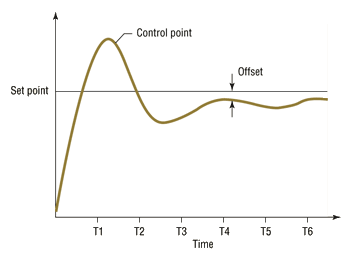
\includegraphics[width=0.5\linewidth]{img/recorrencia-graph.png}
		\label{fig:graph}
		\caption{Representação da atuação do controle sobre o ganho da aceleração e controle de velocidade do carro.}
	\end{figure}



\section{Análise do Funcionamento dos Motores} \label{sec:analitico}
	De forma a adentrar na causa que impediu a conclusão do trabalho, realizou-se testes analíticos a fim de encontrar a causa dos problemas.

	% explicando os intervalos e as situações
	Como o carro necessita de se comportar bem em altas e baixas rotações, analisou-se duas das mais importantes sendo esta quando os motores estão em alta e baixa rotação.% partindo da premissa que o motor inicia-se parado.

	%Para o funcionamento do carro de forma correta, seria necessário o controle proporcional ter gerência de vários intervalos de velocidade, desde a velocidade máxima até a menor, incluindo quando o motor estiver parado. 
	%Ao possuir um intervalo grande de velocidade, permite-se que o carro fizesse curvas com melhor controle evitando as oscilações grandes.
	%Eliminando a situação de quando o motor está parado, para validação, analisou-se das duas ocasiões mais importantes enfrentadas pelo carro, sendo essas quando ele está em alta e baixa rotação. 
	%Esses dados são importantes pelo fato que ambas (alta e baixa rotação) são velocidade extremas do intervalo usado pelo controle e que elas possuem outras variáveis que influenciam na sua atuação como a intensidade da corrente de partida e a resistência dos trens de engrenagem situados em cada motor, por exemplo.

	Para representar essas rotações, foi relacionado os intervalos de valores de PWM da plataforma de protipação. Dessa forma, como o NodeMCU gera um intervalo de 0 à 1023 para valores de PWM, utilizou-se dos valores 1023 e 600 para alta e baixa rotação respectivamente. 
	%O carro que comporte em ambas as situações permite-se concluir que ele possui todos os requisitos físicos necessários para que o controle consiga operar com mais facilidade obtendo melhor precisão em suas tarefas propostas.
	%Assim, o carro que não realizar bem tais movimentos, poderá ter problemas futuros como estabilidade e precisão, por exemplo.

	Neste primeiro teste, partiu-se do princípio que o motor encontra-se parado. Sobre esse aspecto, os itens analisados foram as correntes:

	\begin{description}
		\item [Partida:] Intensidade de corrente que o motor necessita para gerenciar a partida, ou seja, a tentativa de movimento;
		\item [Nominal:] Intensidade de corrente após a tentativa de partida inicial. Valores normativos do motor ao longo do tempo seguindo um mesmo valor de entrada de PWM.
		%\item [Movimento:] Intensidade do motor quando este está realmente realizando o movimento giratório, ou seja, quando realmente conseguiu sair da inércia inicial que é estar sem movimento.
	\end{description}

	Executou-se dez testes mensurando\footnote{Sendo $\bar{X}$ a média, $\sigma$ o desvio padrão e a porcentagem do erro calculado pela fórmula $\frac{\sigma}{\sqrt{|x|}}$ no qual $x$ sendo os total de valores coletados.} os valores de intensidade de corrente em Partida (Tabela \ref{tab:corrente_partida}) e Nominal (Tabela \ref{tab:corrente_nominal}).% e Movimento (Tabela \ref{tab:corrente_rotacionado}).

	\begin{table}[H]
    	\centering
    	\caption{Tabela de valores médios de intensidade de corrente de partida aos principais movimentos requeridos pelo carro robô.}
	    \begin{tabular}{|c||c|c|c|} \hline
	    ~                      & $\bar{X}$ \textbf{Corrente de Partida}   & $\sigma$   & \textbf{\% Erro} \\ \hline \hline
	    \textbf{Alta  Rotação} & $313,7mA$                                & $26,36938$ & $8,338732$    \\ \hline
	    \textbf{Baixa Rotação} & $283,2mA$                                & $19,65706$ & $6,216108$    \\
	     \hline
	    \end{tabular}   \label{tab:corrente_partida}
	\end{table}

	\begin{table}[H]
    	\centering
    	\caption{Tabela de valores médios de intensidade de corrente nominal aos principais movimentos requeridos pelo carro robô.}
	    \begin{tabular}{|c||c|c|c|} \hline
	    ~                      & $\bar{X}$ \textbf{Corrente Nominal} & $\sigma$   & \textbf{\% Erro} \\ \hline \hline
	    \textbf{Alta  Rotação} & $138,9mA$                           & $14,22400$ & $4,498024$     \\ \hline
	    \textbf{Baixa Rotação} & $215,7mA$                           & $11,75727$ & $3,717974$     \\ 
	     \hline
	    \end{tabular}   \label{tab:corrente_nominal}
	\end{table}

	%teste alta velocidade
	%\subsection{Análise da Alta Rotação}
		Olhando primeiramente a alta rotação, o carro possui força suficiente para iniciar seu movimento com a corrente de partida ($313,7mA$) e, depois de vencer a inércia, a corrente estabiliza em valores próximos à $138,9mA$ fazendo o motor girar como estabelecido. 

		Todos os dez testes realizados com este valor de potência fez com que o carro obtivesse teve sucesso para vencer sua inércia inicial. Isso deve-se ao fato da aceleração do motor ser alta, sobrepondo qualquer resistência física que impede o movimento da roda. Diferentemente do teste de alta rotação, o teste com baixa velocidade não obteve tanto sucesso.

	%teste baixa velocidade
	%\subsection{Análise da Baixa Rotação}
		Nos testes de baixa rotação o valor de intensidade de corrente de partida teve uma média de $283,2mA$, mas, em todos os testes realizados, esse valor de potência não foi suficiente para iniciar a rotação no motor. 
		O valor $600$ de PWM fracassou em todos os testes di girar a roda, mesmo o motor demonstrando aplicar a força ao emitir barulho de acionamento. 

		Verificando a dificuldade do início da rotação nos testes de baixa velocidade, foi realizado uma nova medição de valores de corrente nominal com o motor partindo da definição que eles já estávam em movimento. Assim, obteve os resultados da Tabela Movimento (Tabela \ref{tab:corrente_rotacionado}).
		%uma pequena ajuda manual à roda para o giro inicial e percebeu que, para este giro inicial, o motor aplica uma força suficiente para a movimentação do carro mas insuficiente para vencer a resistência dos trens de engrenagens da caixa de redução.


	\begin{table}[H]
    	\centering
    	\caption{Tabela de valores médios de intensidade de corrente com o motor rotacionando aos principais movimentos requeridos pelo carro robô.}
	    \begin{tabular}{|c||c|c|c|} \hline
	    ~                      & $\bar{X}$ \textbf{Corrente c/ Motor em Rotação} & $\sigma$   & \textbf{\% Erro} \\ \hline \hline
	    \textbf{Alta  Rotação} & $142,0mA$                                         & $5,656854$ & $1,788854$     \\ \hline
	    \textbf{Baixa Rotação} & $130,8mA$                                         & $18,68927$ & $5,910067$     \\ 
	     \hline
	    \end{tabular}   \label{tab:corrente_rotacionado}
	\end{table}

	Tabela \ref{tab:corrente_rotacionado} exibe valores mais baixos de corrente nominal partindo do pressuposto de que o motor já estava girando. 
    
	Em teoria, a baixa rotação deveria ser acionada, o motor iniciar seu giro e a rotação estabilizada com valores de intensidade de corrente nominal $I_{nominal} = 130,8$. Entretanto, a corrente de partida $ I_{partida} = 283,2$ não é suficiente para iniciar a movimentação do carro. Dos testes realizados com propósito do motor conseguir dar a partida, necessitou-se de intensidades de correntes maiores que $I_{giro} = 311,1$ para obter seu início. Isso da uma diferença de corrente de $I_{diferenca\_partida} = 27,9mA$, ou seja $10,1505\%$ de potência a mais para as rotações tendo o PWM em valores próximos de $665$.
    
    Na Seção \ref{sec:discussao} será feita uma discussão sobre os dados coletados em relação à atuação do carro.

	\subsection{Discussão} \label{sec:discussao}
		%Após os testes, percebeu-se alguns problemas principais no projeto sendo eles: 1) Resistência das engrenagens da caixa de redução; e 2) Torque fraco dos motores. Eles serão descritos a seguir.

		%  peso do carro
		%O primeiro problema é o \todo{peso} do carro. Ao adicionar todos os componentes para seu funcionamento, percebeu-se que o carro possui \todo{peso} elevado. Os motores possuem força o suficiente para realizar o movimento do carro, mas com \todo{peso} elevado, o controle terá maior dificuldade de controlar a partida dos motores e a estabilização da velocidade.

		\subsubsection{Trens de Engrenagens da Caixa de Redução}
			% engrenagens

			%comparacao
			%Dessa forma, sabendo de tais problemas físicos do carro, realizou-se uma análise das situações mais importantes que o robô enfrenta com base em movimento teóricos perfeitos que fariam o carro realizar a tarefa proposta com sucesso.
			

			Feito a análise de correntes, percebeu-se que existe uma grande resistência das caixas de reduções para início de rotação.
			Esse problema físico foi perceptível ao visualizar a situação na qual o motor injetava potência para iniciar o giro e não conseguia. Pensou-se de início que a potência acionada era insuficiente para a movimentação do carro, entretanto, no teste com o carro já em movimento, o valor mostrou-se suficiente para mover o carro com todos os componentes instalados com facilidade. Assim, a potência é suficiente para arrastar o carro, mas não para dar sua partida.
			Houve situações de execução fora dos testes em que o carro injetou potência máxima nos motores (valor $1023$ de PWM) e eles não conseguiam se mover.

			% problema da engrenagens resolvidas pelo controle
			Esse problema poderia ser resolvido pelo controle, acionando mais potência no início e depois equilibrando no início de seu movimento. Entretanto, esse procedimento não foi possível ser implementado por vários motivos sendo eles:

			\begin{enumerate}
				\item Injetar mais potência na partida faz com que sua aceleração seja alta de tal forma que, após iniciada, o controle não consiga corrigí-la. Isso é causado pelo item mencionado em Seção \ref{sec:problema_motor} no qual é descrito um certo atraso na atuação do motor, podendo causar descontrole de seus movimentos e consequentemente a perdendo o caminho a seguir. Sendo assim, a primeira solução sobre o problema da resistência foi adicionar mais pares de motores ao carro, entretanto, o chassi do carro não possui suporte para a instalação de mais motores com seus \textit{encoders};

				% valores altos de potência fazem o carrinho perder o controle
				\item O carro ter que percorrer $9\degree$ (ou seja, $0,5105$ centímetros) para que o controle note o início do movimento também é um fator que torna o problema complexo. 
				Essa distância percorrida somada com o tempo processamento do carro ($30$ milissegundos), do processamento da nuvem e sua a latência de comunicação de envio e do recebimento de dados até a atuação do controle faz com que o carro percorra cerca de $0,742$ centímetros até que a atuação seja totalmente completada. 
				
                Esse valor de distância é suficiente para fazer com que o carro não consiga recuperar de uma situação que exija mais potencial do controle. O problema poderia apresentar uma solução ao utilizar um disco para \textit{encoder} com mais vasos criando uma precisão maior dos movimentos, mas não havia tal equipamento para uso. Esse problema de controle de aceleração torna mais problemático ainda no carro $ \mathcal{B} $ pois:

				\begin{itemize}
					\item Como ele não possui um item de controle de posição geral de trajeto, o carro fica a mercê da precisão exercida pelo controle junto com os valores obtidos com o \textit{encoder}. Com um controle de aceleração dado pelos fatores acima, cada movimento do carro acumula erros exponencialmente. De uma maneira mais geral, a cada movimento é gerado um erro que é aplicado no próximo movimento e assim gerado um novo erro com valor exponencialmente maior, criando assim uma bola de neve e inviabilizando a reprodução do carro $ \mathcal{B} $.
				\end{itemize}
			\end{enumerate}


\section{Conclusão} \label{sec:conclusao}

	Como produto do trabalho, o carro $ \mathcal{A} $ consegue completar o trajeto com algumas dificuldades mesmo o processamento situar todo em nuvem. Entretanto, o carro $ \mathcal{B} $ não conseguiu realizar nenhuma vez sua tarefa de reprodução do trajeto realizado por $ \mathcal{A} $. Isso pois não foi possível neste trabalho a construção de um modelo que levasse em consideração o fator de erro do $ \mathcal{B} $ em relação ao trajeto.

	Como demostrativo do funcionamento do carro $ \mathcal{A} $, segue os \textit{links} disponibilizou-se três vídeos para exemplificar o funcionamento do carro. O primeiro vídeo \url{https://youtu.be/RWjgYUrU1Fo} exibe o carro realizando seu dever de completar o trajeto. O mesmo vídeo pode ser visto em câmera lenta, gravado em $240fps$ percebendo cada detalhe do carro e seu procedimento de controle, disponível em \url{https://youtu.be/xk-tbqkAVOs}. Também foi disponibilizado um vídeo demonstrando o tempo de demora na atuação dos motores após a leitura da faixa no qual pode ser verificado em câmera lenta, disponibilizado em \url{https://youtu.be/pGvHHe4h54I}. Por fim, outro vídeo (com música de fundo) demonstrando outra atuação do carro, disponível em \url{https://youtu.be/SD5c9YnoTfo}. Como mencionado, não há demonstração do carro $ \mathcal{B} $ pois todos os testes realizados com tal foram falhos.

	% tempo de resposta
    Após analisado os componentes em conjunto com a atuação do controle proporcional do carro, percebeu-se que a latência de resposta do motor em virtude ao intervalo de resposta esperado pelo controle faz com que o carro não tenha uma precisão fina sobre seus movimentos. Esse problema poderia ser reduzido ao utilizar abordagem que passasse a utilizar um processamento de controle totalmente local tornando o processamento mais preciso.
    
	% mais tricks seria legal
	Utilizar um \textit{encoder} que contenha mais vasos faz com que seja criado uma maior percepção de movimento, fazendo com que o controle gerencie melhor a velocidade do carro. 
    O modelo atual utilizado usa apenas 3 valores de velocidade pelo fato do tempo curto de captura de taxa de variação de \textit{tricks} criando curta amostra de velocidade. Com um disco com mais vasos, é possível multiplicar o nível de precisão de seus movimentos.

	% engrenagens
	Mesmo com torque suficiente para mover-se em baixas rotações, o motor não conseguiu vencer à resistência dos trilhos de engrenagens em situações onde o carro encontrava-se estacionado. Como mencionado na Seção \ref{sec:discussao}, aumentar a aceleração de fato faz o carro dar a partida, mas isso acarreta vários outros problemas relacionados a aceleração. Para garantir acelerações suaves, seria necessário utilizar um sistema de engrenagens que não obtivesse tanta resistência ou motores que tivesse uma capacidade de torque maior.

	% peso}
	%Obviamente, utilizar componentes mais leves faz com que o carro tenha mais facilidade de movimentação dispondo menos resistência aos motores. Quanto menor a resistência enfrentadas pelos motores, mais será a eficiência energética e e seu fator de controle.

	% novo chassi
	%Propor um trabalho fornecendo um chassi que tenha suporte à mais motores e seus \textit{encoders} faz com que o trabalho possa ser desmembrado em mais opções de construções. Alterar a estrutura física do carro, adicionando mais motores por exemplo, faz com que o desenvolvimento do carro seja abordado de mais formas, escolhendo a que mais atrela ao ambiente testado e equipamentos disponibilizados.


	%O carro $ \mathcal{A} $ consegue completar o trajeto com muita dificuldade pela quantidade de sensores que o carro possui, incluindo seus chassis, rodas, motores, controlador etc. A fim de contornar esse problema, implementou-se um controlador que fosse capaz de lidar com esse problema de atuação dos motores obrigando o carro parar a cada momento que encontra uma faixa, já que este fica impossibilitado de movimentar mesmo utilizando dois \textit{packs} de pilhas com um total de $6V$ cada. 

	% dificuldades
    \subsection{Dificuldades e Ganhos de Aprendizagem}
	Todos os dois \textit{motor shield} fornecidos para o trabalho possuíam problema de circuito físico no qual, o seu componente \textit{not}, que permitia o motor girar em sentido contrário, estavam danificados. Não se sabe o motivo da danificação. Gastou-se muito tempo descobrindo a falta deste circuito integrado e por isso o projeto foi fundado sobre o \textit{motor shield} incapacitado de girar os motores em sentido reverso.

	A geração de um mapa para o carro $ \mathcal{B} $ também foi uma tarefa incompleta. Realizou-se várias tentativas de geração e reprodução de mapas utilizando várias combinações de sensores, mas todas foram fracassadas.

	% Utilização de controles mais eficientes
	O controle proporcional (P) desenvolvido neste trabalho foi capaz de concluir o objetivo do carro $ \mathcal{A} $ mas com dificuldade. É possível realizar um novo estudo a fim de utilizar controle proporcional integral-derivativo (PID) a fim de aprimorar os movimentos dos carros.

	% ganhos
	Neste trabalho foi possível perceber a importância dos controles proporcionais de primeira ordem. Este exemplo de \textit{follow line} do trabalho mostrou-se claro ao comparar as vantagens de sua utilização para obter melhores resultados na sua tarefa. 
    Esse trabalho tornou-se extremamente útil na percepção da qual vários outros sistemas poderiam tomar proveito do uso de tais ferramentas para controle de suas tarefas com maior precisão.
	Outro tópico também aprendido na realização deste trabalho foi o aperfeiçoamento das técnicas básicas de confecção, manuseio e aferição de circuitos eletrônicos simples. Foi necessário conhecimentos básicos sobre corrente elétrica, teoria de circuitos eletrônicos e operação com algumas funcionalidades do multímetro para a construção do trabalho.

\section{Anexos} \label{sec:anexo}
	\subsection{Imagens do Carro Montado}

		\begin{figure}[h]
			\centering
			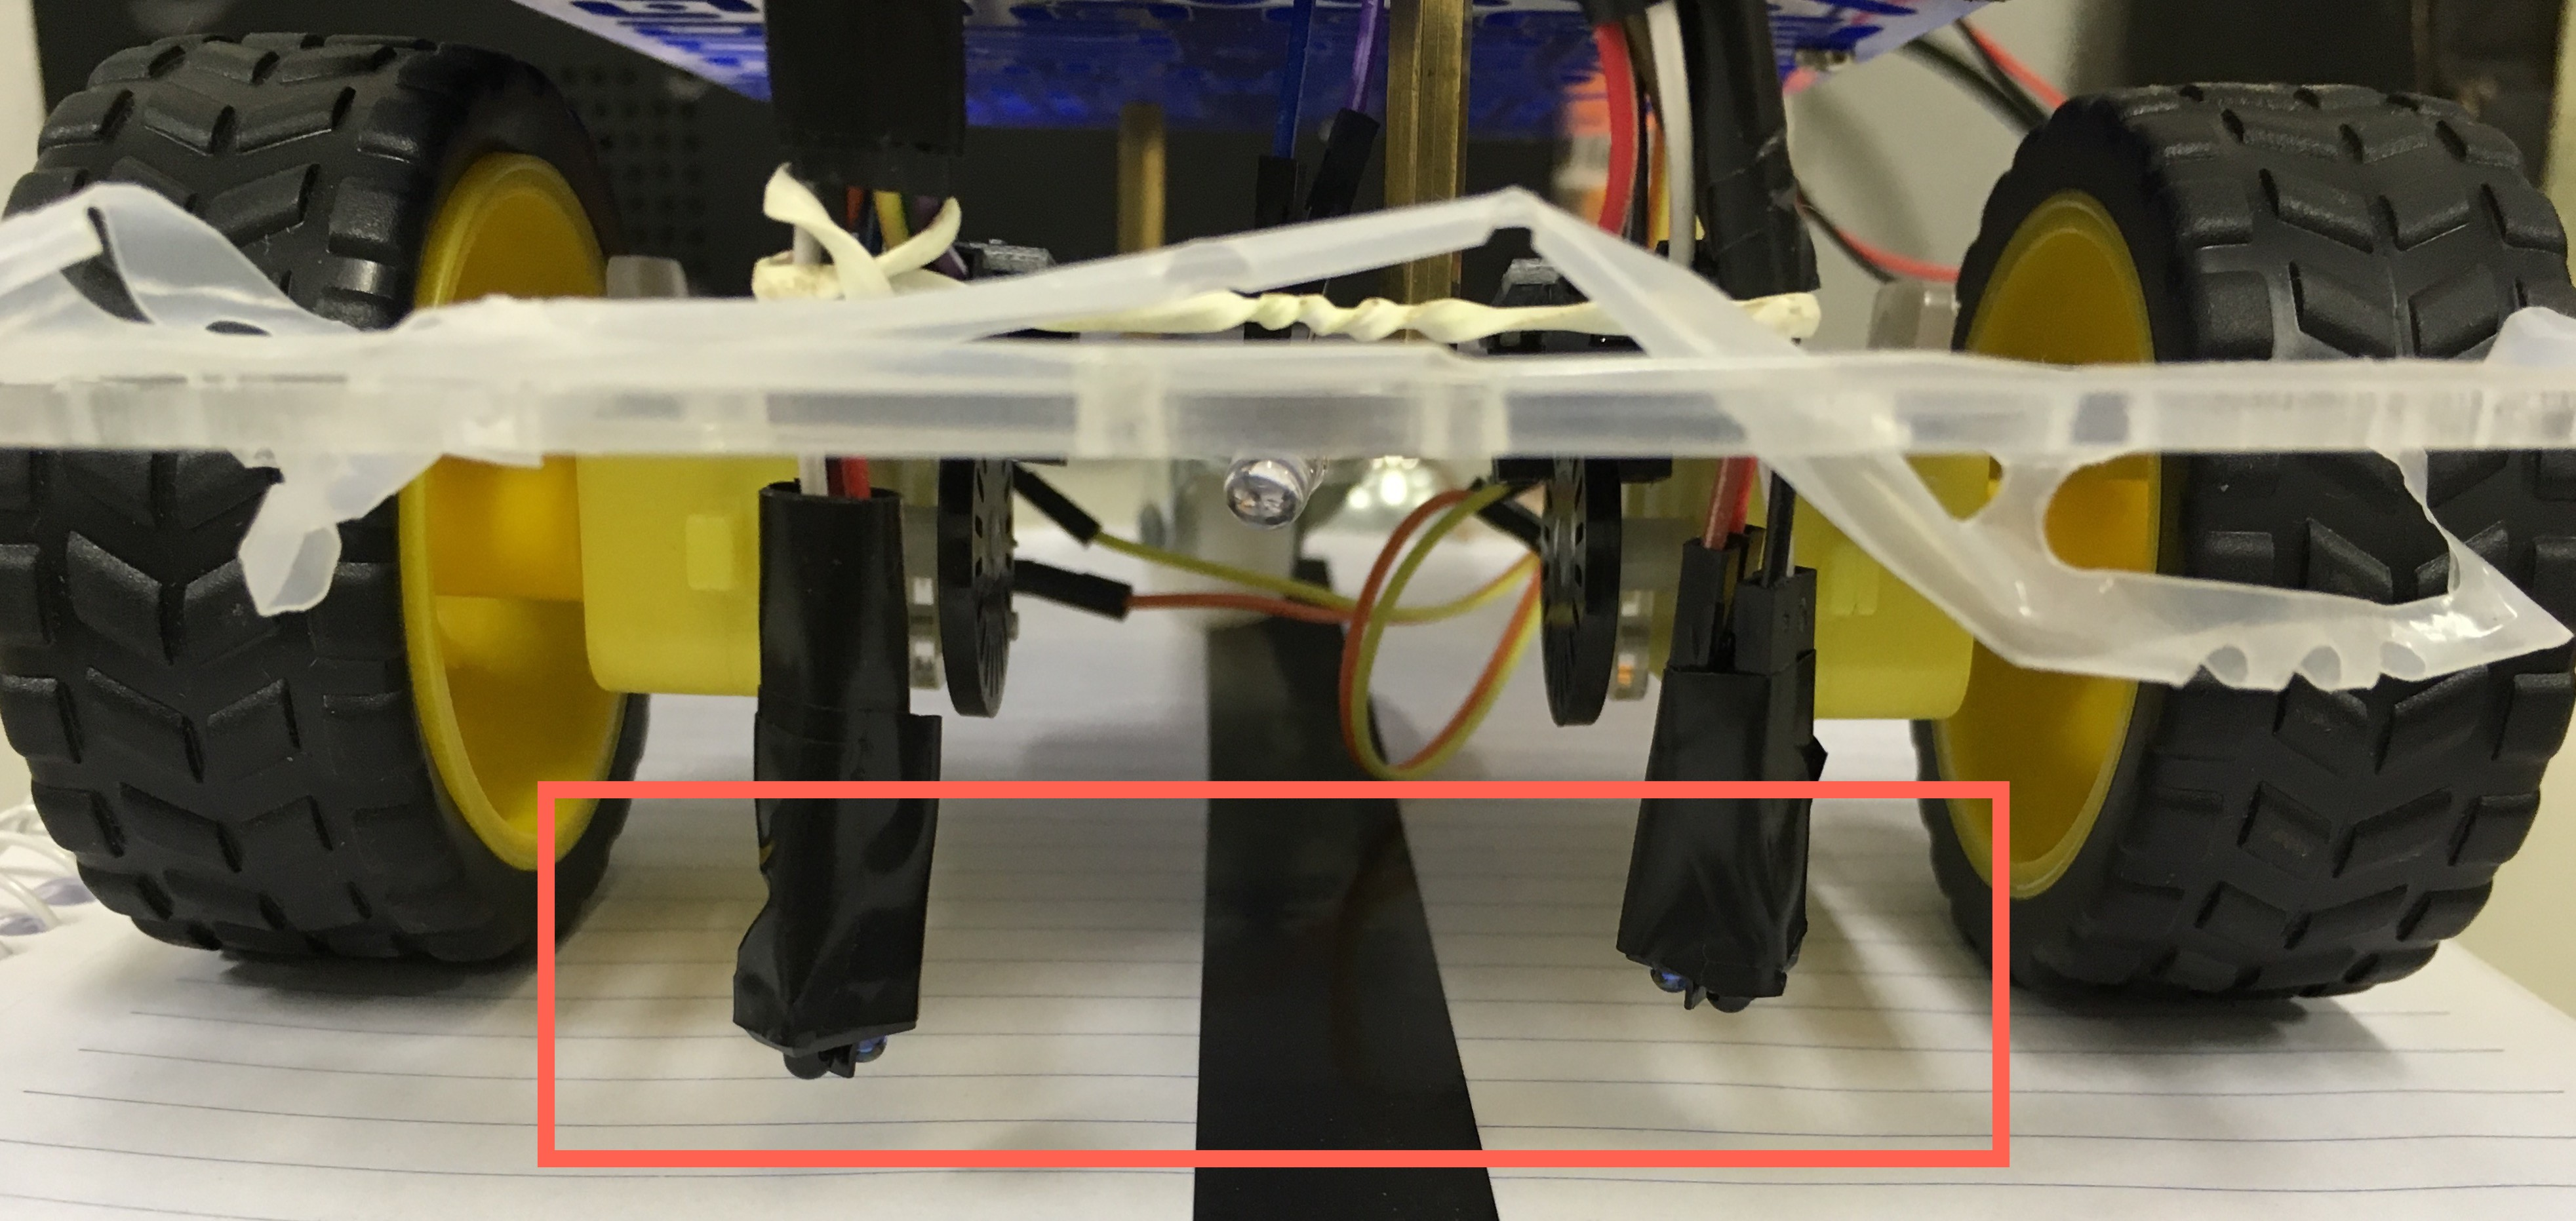
\includegraphics[width=1\linewidth]{img/robot_fotos.jpg}
			\label{fig:robot_foto}
			\caption{Carro Robô $ \mathcal{A} $ e os sensores fototransistores.}
		\end{figure}

		\begin{figure}[h]
			\centering
			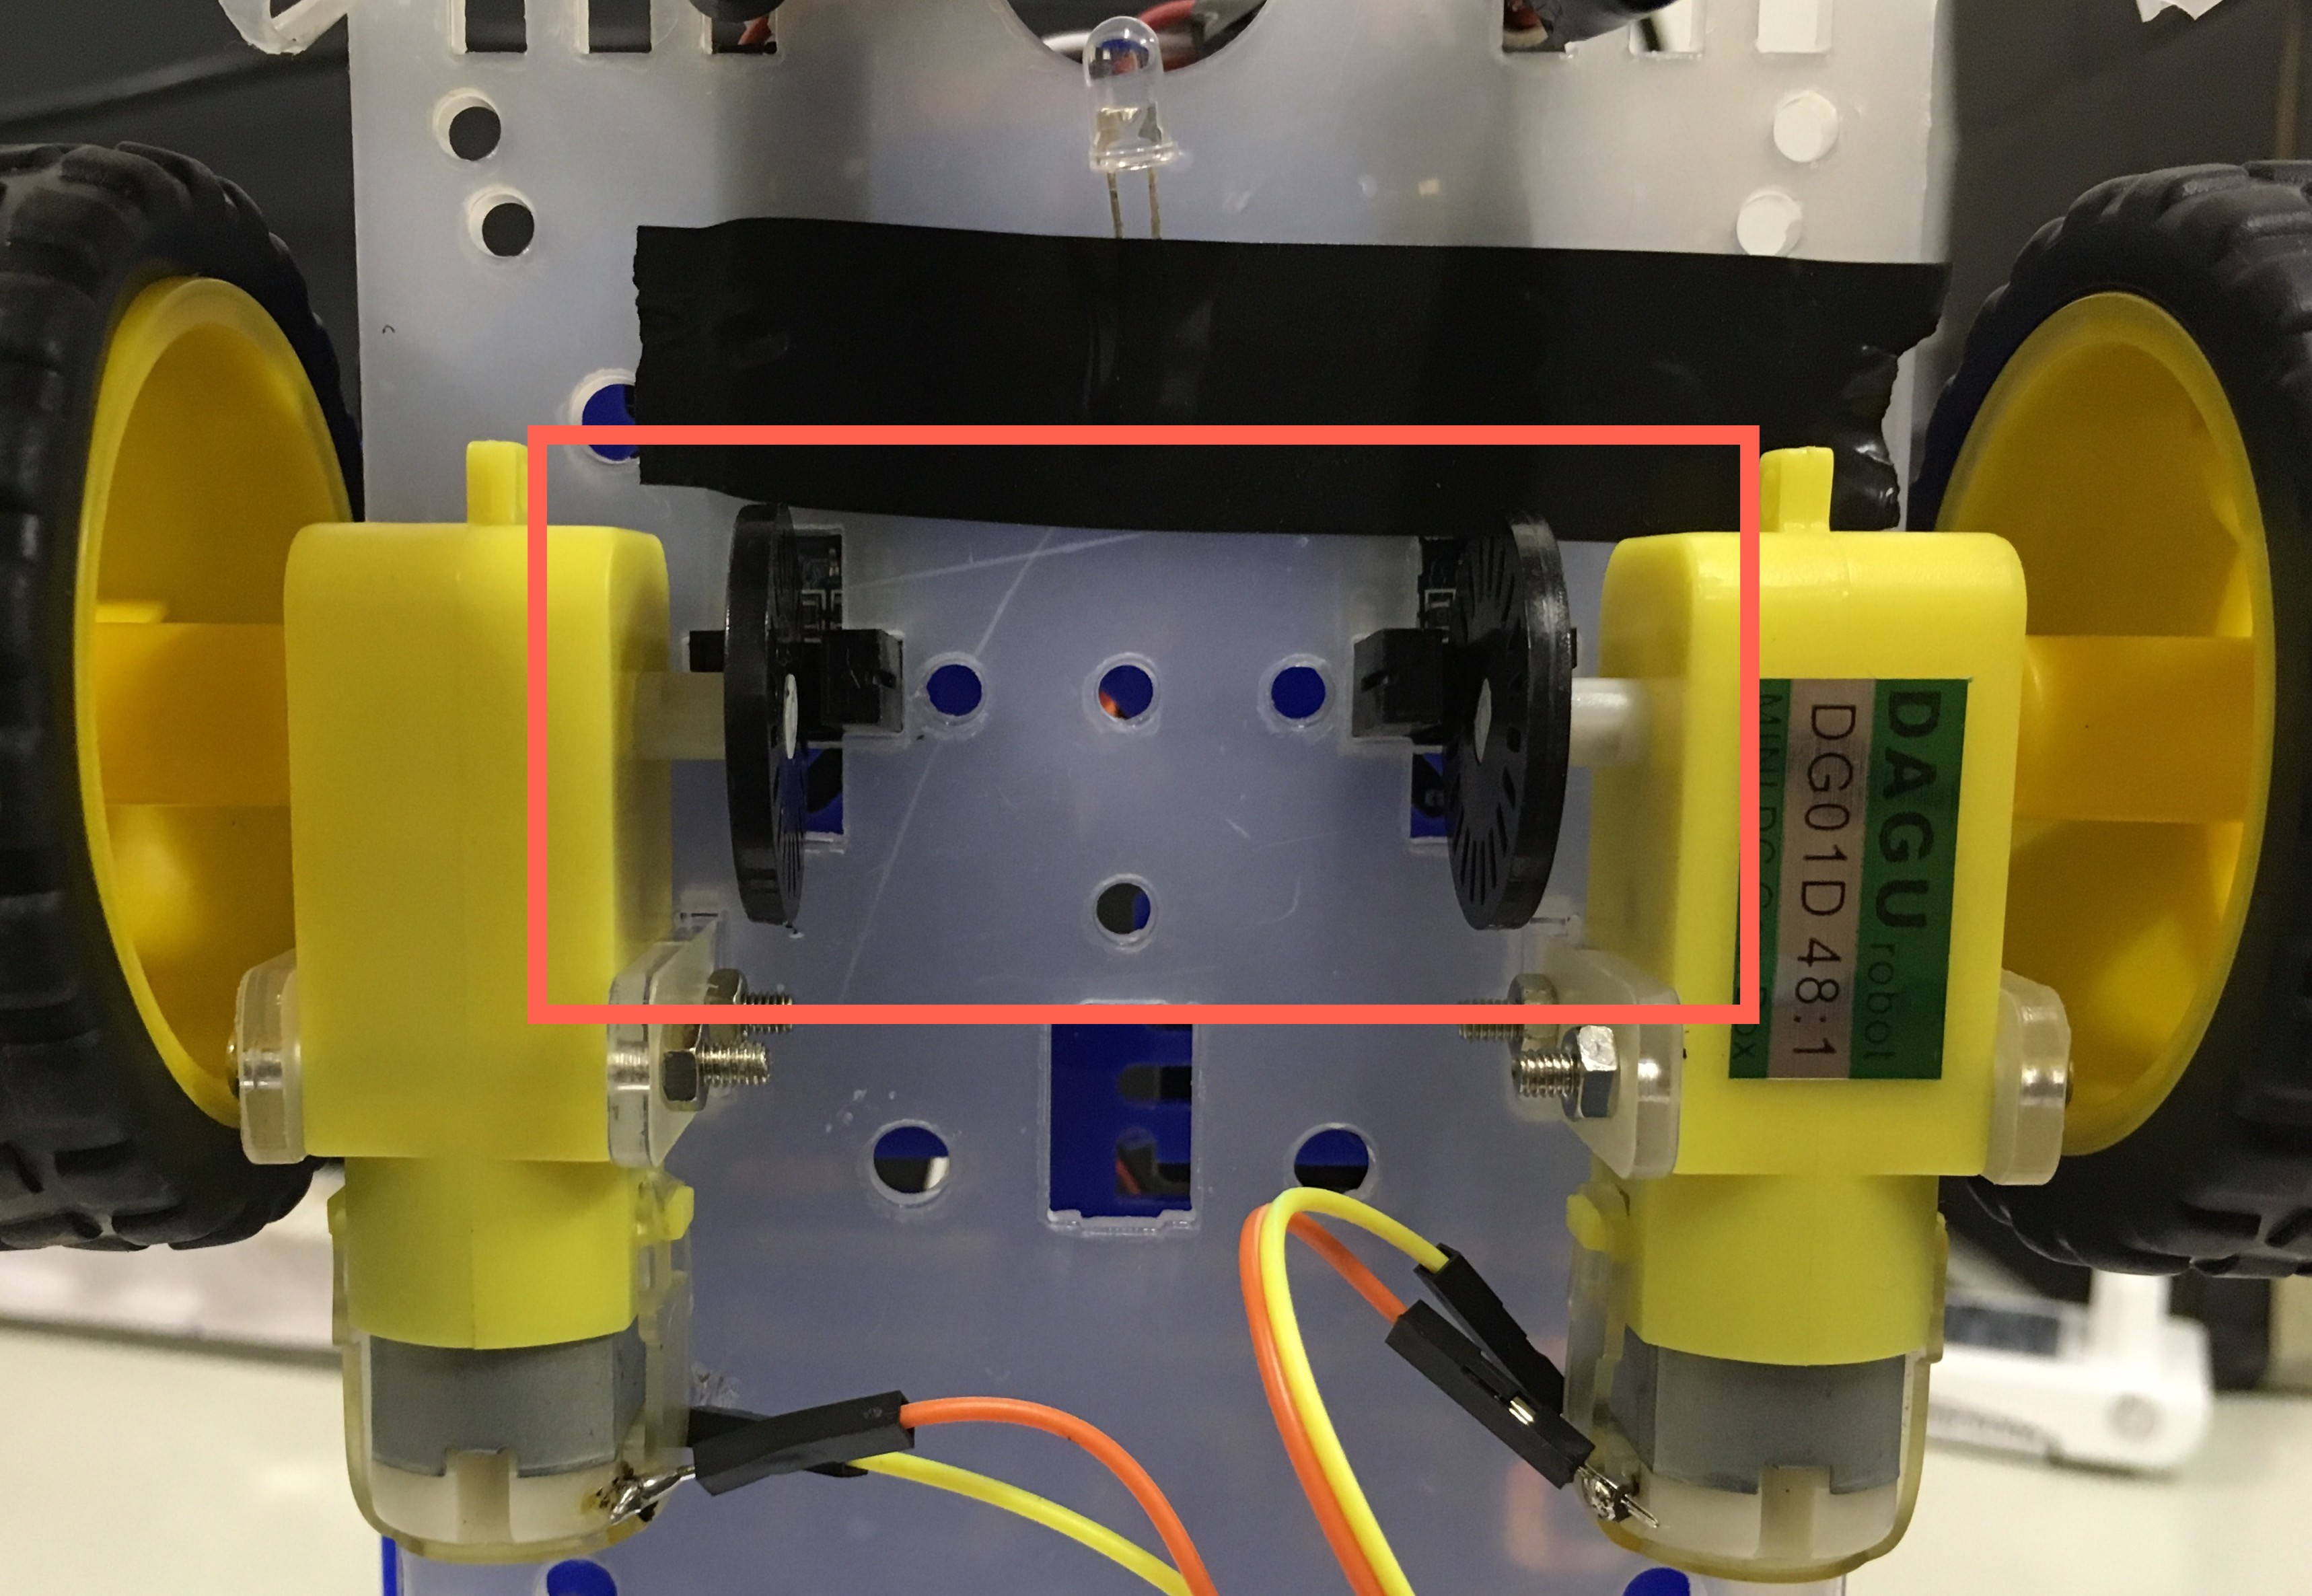
\includegraphics[width=1\linewidth]{img/robot_encoders.jpg}
			\label{fig:robot_encoder}
			\caption{Carro Robô $ \mathcal{A} $ e os sensores encoders.}
		\end{figure}
        
		\begin{figure}[ht]
			\centering
			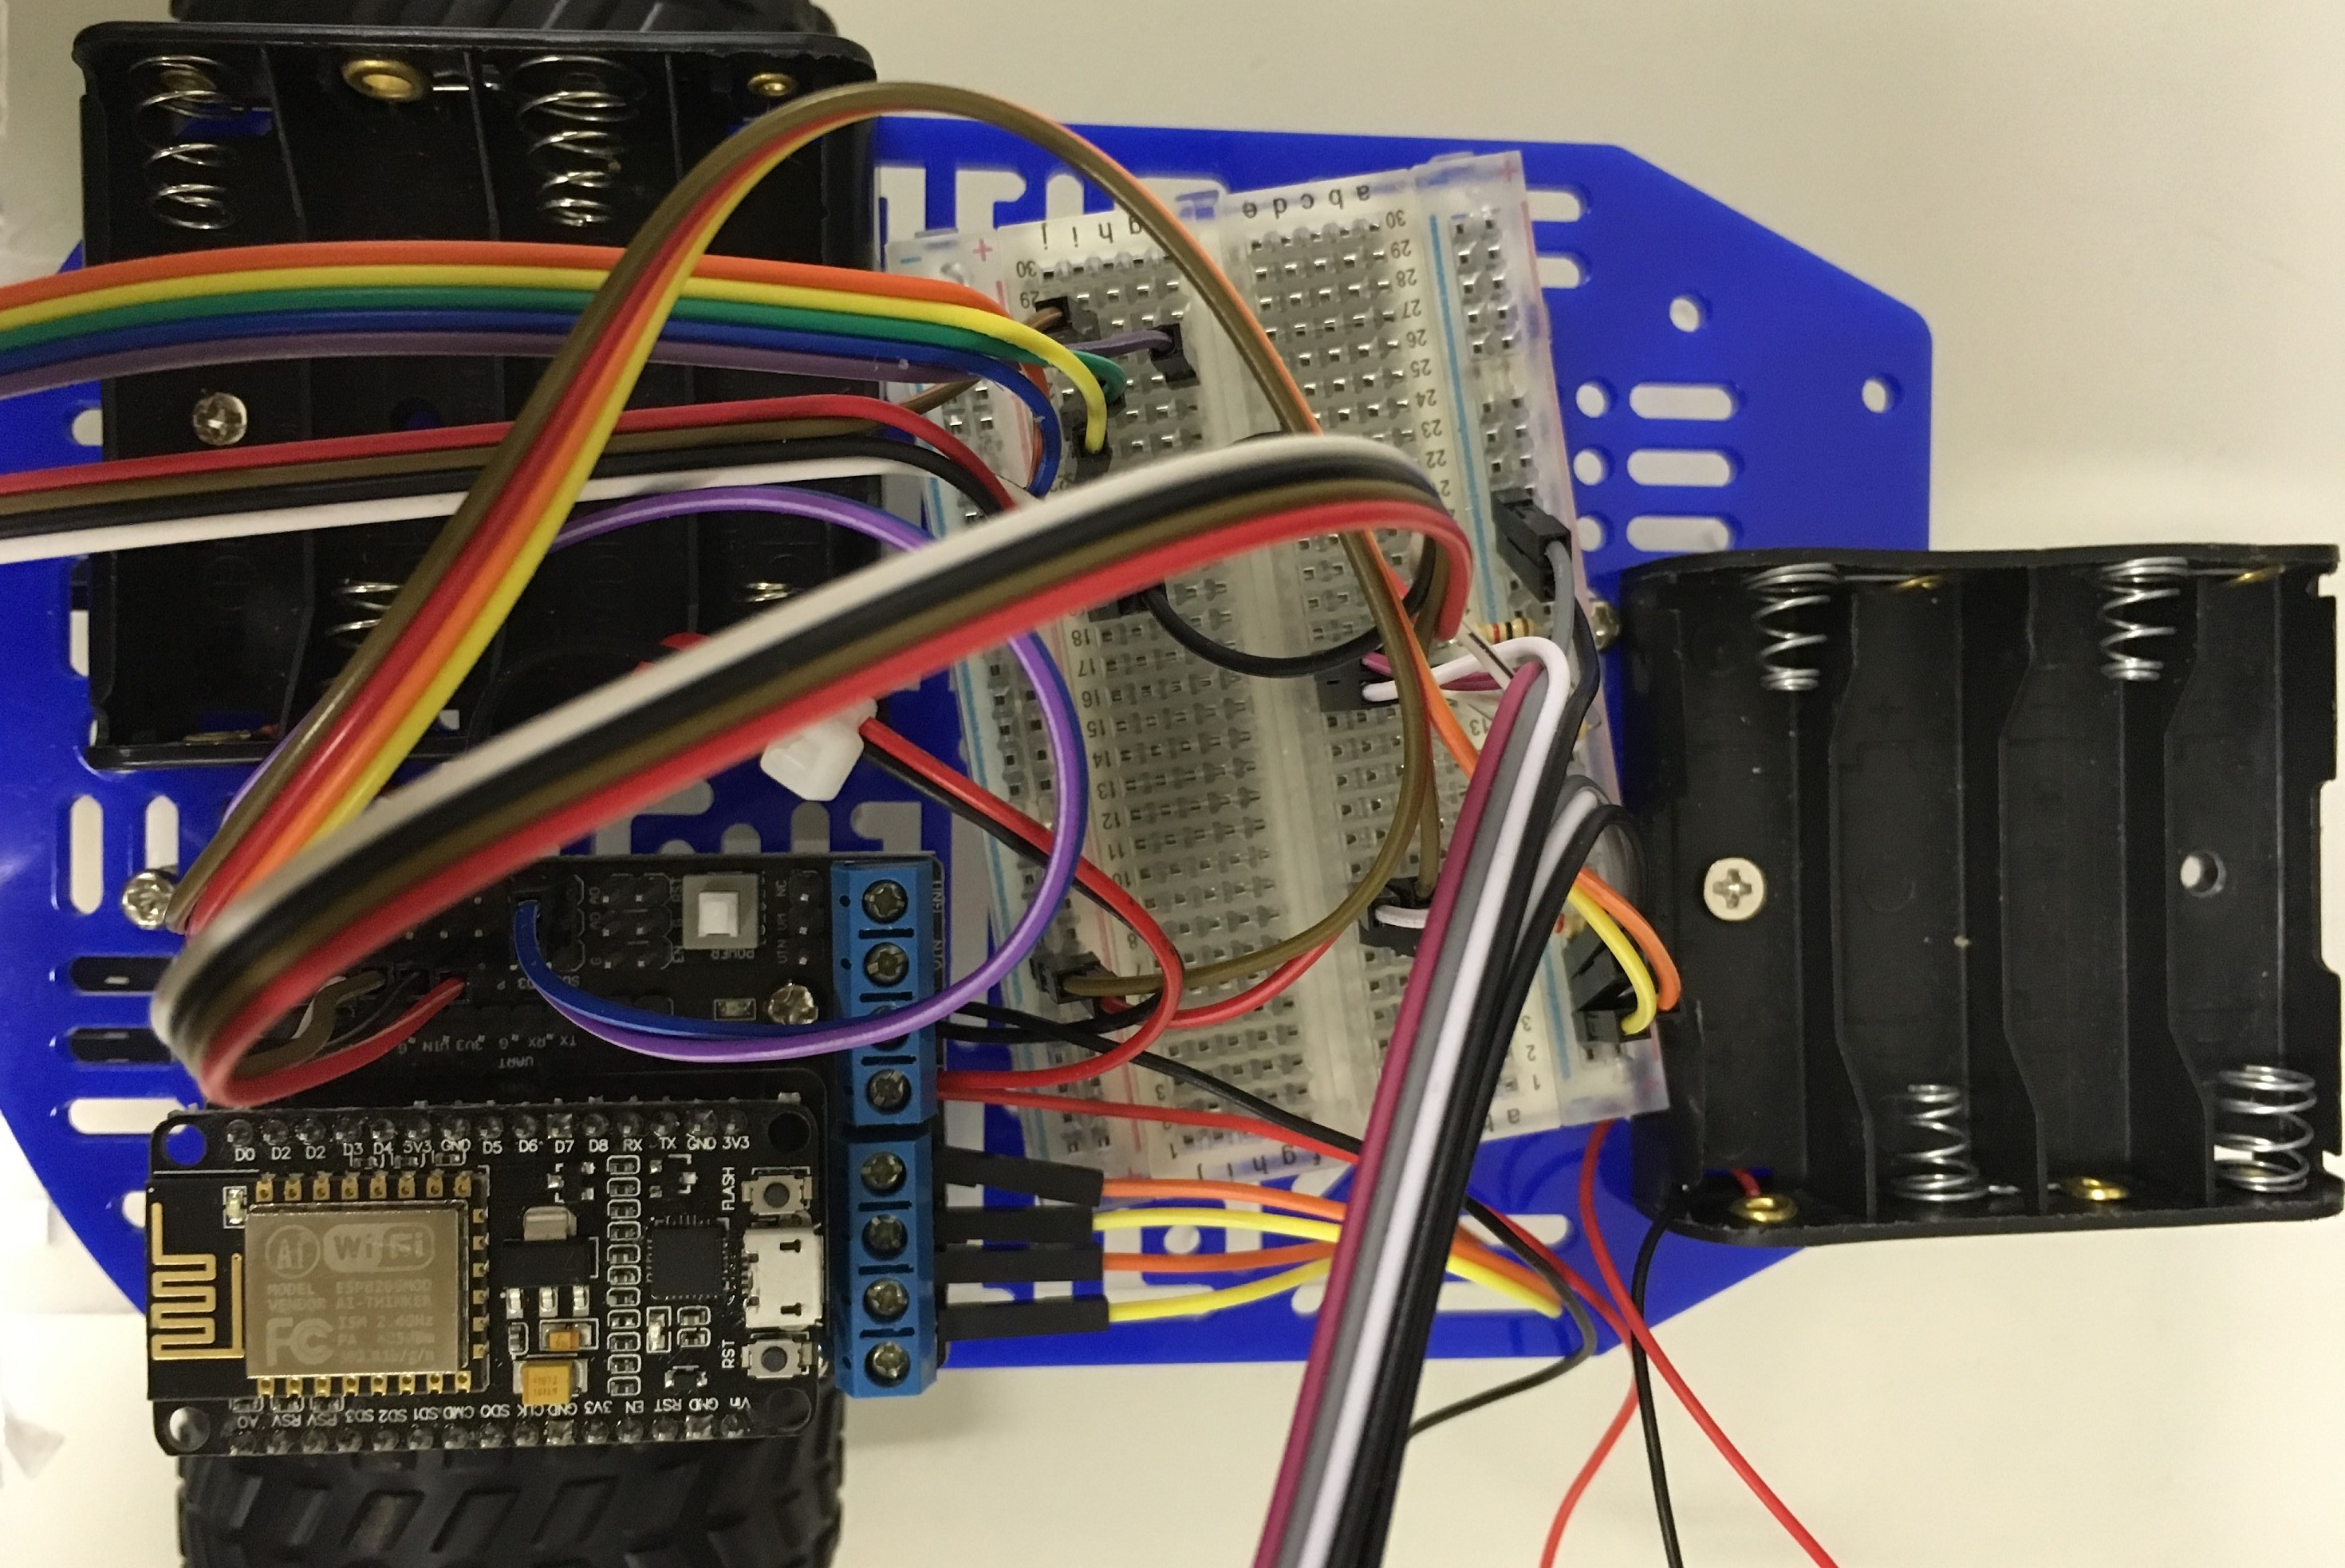
\includegraphics[width=1\linewidth]{img/robot.jpg}
			\label{fig:robot}
			\caption{Carro Robô $ \mathcal{A} $.}
		\end{figure}
		
	\subsection{Código em Linguagem Arduino}
	\subsubsection{ploudy NodeMCU}
		\begin{minted}
			[
			frame=lines,
			framesep=2mm,
			tabsize=3,
			breaklines=true,
			baselinestretch=1.2,
			fontsize=\scriptsize,
			linenos
			]{c++}
#include <SoftwareSerial.h>
#include <stdio.h>
#include <ESP8266WiFi.h>
#include <Wire.h>
#include "MPU9250.h"



// =============== Constants ===================================
#define RADIUS        3.4
#define LARGURE       13.42
#define NUMBER_FRAMES 40
#define DELTA_TEMPO   75
#define SERIALDEBUG   true        
#define SSID          "Imobilis"
#define SSID_PASSWORD "bolinha de sabao"
#define URL           "192.168.0.174"
#define PORT          8888

// =============== Instantiations ==============================
WiFiClient client;
MPU9250 accelgyro;
I2Cdev   I2C_M;
// =============== Variables for MPU9250 =======================
#define sample_num_mdate  5000
volatile float mx_sample[3], my_sample[3], mz_sample[3];
static float mx_centre = 0, my_centre = 0, mz_centre = 0;
static float mx_max = 0, my_max = 0, mz_max = 0;
static float mx_min = 0, my_min = 0, mz_min = 0;
uint8_t buffer_m[6];
int16_t mx, my, mz;
float heading;
float Mxyz[3];
// =============== Human Interface and Controls ================
char command         = '0';
bool restart_program = true;
// =============== Pins ========================================
long pin_left_motor_pwm           = D1;  // Pin to left motor pwm          
long pin_righ_motor_pwm           = D2;  // Pin to righ motor pwm          
long pin_left_motor_pwm_direction = D3;  // Pin to left motor direction
long pin_righ_motor_pwm_direction = D4;  // Pin to righ motor direction
long pin_left_optical_sensor      = D5;  //Pin to optical sensor
long pin_righ_optical_sensor      = D6;  //Pin to optical sensor
long left_encoder                 = D7;  // Pin to encoder
long righ_encoder                 = D8;  // Pin to encoder
// =============== Timing ========================
unsigned long tempo               = 0;
unsigned long global_start_time   = 0;
unsigned long global_spended_time = 0;
// =============== Send Datas =================
byte left_light_boolean = 1, righ_light_boolean = 1;
byte left_light_boolean_inter = 1, righ_light_boolean_inter = 1;
// =============== Receive Datas =================
long size_map       = 0;
char s_package[256] ;
bool package_sent   = false;
String str_send     = "";

//TODO: Rever essas variáveis se estão postas de forma certa
int left_master_pwm    = 0;
int righ_master_pwm    = 0;
int left_master_frames = 0;
int righ_master_frames = 0;

// =============== Encoder Angular Velocity ====================
long left_current_encoder_this_car = 0;
long righ_current_encoder_this_car = 0;
long left_last_encoder_this_car    = 0;
long righ_last_encoder_this_car    = 0;
long x_point                       = 0;
long y_point                       = 0;
int reference                      = 0;




 float calculating_heading(void) {
	heading = 180 * atan2(Mxyz[1], Mxyz[0]) / PI;
	if (heading < 0) heading += 360;

	return heading;
}

void getTiltHeading(void) {
	float pitch = asin(-Axyz[0]);
	float roll = asin(Axyz[1] / cos(pitch));

	float xh = Mxyz[0] * cos(pitch) + Mxyz[2] * sin(pitch);
	float yh = Mxyz[0] * sin(roll) * sin(pitch) + Mxyz[1] * cos(roll) - Mxyz[2] * sin(roll) * cos(pitch);
	float zh = -Mxyz[0] * cos(roll) * sin(pitch) + Mxyz[1] * sin(roll) + Mxyz[2] * cos(roll) * cos(pitch);
	tiltheading = 180 * atan2(yh, xh) / PI;
	if (yh < 0)    tiltheading += 360;
}


void Mxyz_init_calibrated () {
	Serial.print("\n[INFO] Sample starting......");  
	Serial.print("\n[INFO] waiting ......");

	get_calibration_Data ();

	Serial.print("[INFO] Compass calibration parameter: ");
	Serial.print(mx_centre); Serial.print(", ");
	Serial.print(my_centre); Serial.print(", ");
	Serial.print(mz_centre);
}


void get_calibration_Data () {

	get_one_sample_date_mxyz();
	mx_max = mx_sample[2];
	my_max = mx_sample[2];
	mz_max = mx_sample[2];
	mx_min = mx_sample[2];
	my_min = mx_sample[2];
	mz_min = mx_sample[2];

	for (int i = 0; i < sample_num_mdate; i++) {
		get_one_sample_date_mxyz();

		Serial.print("\n");
		Serial.print(i); Serial.print(":");
		Serial.print(sample_num_mdate); Serial.print("   ");
		Serial.print(mx_sample[2]); Serial.print(" ");
		Serial.print(my_sample[2]); Serial.print(" ");
		Serial.print(mz_sample[2]);

		if (mx_sample[2] >= mx_max) mx_max = mx_sample[2];
		if (my_sample[2] >= my_max) my_max = my_sample[2];
		if (mz_sample[2] >= mz_max) mz_max = mz_sample[2];
		if (mx_sample[2] <= mx_min) mx_min = mx_sample[2];
		if (my_sample[2] <= my_min) my_min = my_sample[2];
		if (mz_sample[2] <= mz_min) mz_min = mz_sample[2];

	}
	mx_centre = (mx_max + mx_min) / 2;
	my_centre = (my_max + my_min) / 2;
	mz_centre = (mz_max + mz_min) / 2;
}

void get_one_sample_date_mxyz() {
	getCompass_Data();
	mx_sample[2] = Mxyz[0];
	my_sample[2] = Mxyz[1];
	mz_sample[2] = Mxyz[2];
}

void getCompass_Data(void) {
	I2C_M.writeByte(MPU9150_RA_MAG_ADDRESS, 0x0A, 0x01); //enable the magnetometer
	delay(10);
	I2C_M.readBytes(MPU9150_RA_MAG_ADDRESS, MPU9150_RA_MAG_XOUT_L, 6, buffer_m);

	mx = ((int16_t)(buffer_m[1]) << 8) | buffer_m[0] ;
	my = ((int16_t)(buffer_m[3]) << 8) | buffer_m[2] ;
	mz = ((int16_t)(buffer_m[5]) << 8) | buffer_m[4] ;

	Mxyz[0] = (double) mx * 1200 / 4096;
	Mxyz[1] = (double) my * 1200 / 4096;
	Mxyz[2] = (double) mz * 1200 / 4096;
}

void getCompassDate_calibrated () {
	getCompass_Data();
	Mxyz[0] = Mxyz[0] - mx_centre;
	Mxyz[1] = Mxyz[1] - my_centre;
	Mxyz[2] = Mxyz[2] - mz_centre;
}


float get_heading() {
    getCompassDate_calibrated();
    return calculating_heading();
}


//          10-DOF
// ===================================================================================================================
// ===================================================================================================================
//          PROCEDIMENTOS ENCODER


int difference_trick_encoder_left() { 
	int diff = left_current_encoder_this_car - left_last_encoder_this_car; 

	if (diff > 8) 
		diff = 0;

	left_last_encoder_this_car = left_current_encoder_this_car;
	return diff;
}
int difference_trick_encoder_righ() { 
	int diff = righ_current_encoder_this_car - righ_last_encoder_this_car; 

	if (diff > 8) 
		diff = 0;

	righ_last_encoder_this_car = righ_current_encoder_this_car;
	return diff;
}

float left_distance_centimeters() { return 2 * PI * RADIUS * (difference_trick_encoder_left()) / NUMBER_FRAMES ; }
float righ_distance_centimeters() { return 2 * PI * RADIUS * (difference_trick_encoder_righ()) / NUMBER_FRAMES ; }

float center_distance_centimeters() { return (righ_distance_centimeters() + left_distance_centimeters()) / 2.0; }


float refresh_x_point() { x_point = x_point + center_distance_centimeters() * cos(reference);   return x_point; }
float refresh_y_point() { y_point = y_point + center_distance_centimeters() * sin(reference);   return y_point; }
float refresh_reference() { reference = righ_distance_centimeters() - left_distance_centimeters() /
 LARGURE;    return reference; }


//          DEFINIÇÕES DE VARIÁVEIS
// ===================================================================================================================
// ===================================================================================================================
//          CONEXÕES DE REDE


unsigned long millis_now() { return millis() - global_start_time; }

void left_add_encoder() { left_current_encoder_this_car++; }
void righ_add_encoder() { righ_current_encoder_this_car++; }

void left_interrupt_ligth() { left_light_boolean_inter = 1; }
void righ_interrupt_ligth() { righ_light_boolean_inter = 1; }

// Função para iniciar a Conexão com a rede WiFi
void start_connection_wifi() {
	bool twice = false;
	do {
		if (SERIALDEBUG && ! twice) {
			Serial.print("\n[INFO] Connecting in: ");
			Serial.print(SSID); 
		}

		WiFi.begin(SSID, SSID_PASSWORD); // connecta na Rede Wireless

		while (WiFi.status() != WL_CONNECTED) {
			if (SERIALDEBUG && ! twice) 
				Serial.print("\n\tNão Conectado na Rede WiFi");
			delay(200);
			twice = true;
		}

		if (SERIALDEBUG) {
			Serial.print("\n[INFO] Conectado na Rede: \n\t");  Serial.print(SSID);
			Serial.print(" | IP ");
			Serial.print(WiFi.localIP());
		}

	} while (WiFi.status() != WL_CONNECTED);
}

void master_connection_cloud() {
	bool twice = false;
	do {
		if (SERIALDEBUG && ! twice) {
			Serial.print("\n[INFO] Start Cloud Connecting");
			Serial.print("\n\tAddress: ");
			Serial.print(URL); 
			Serial.print(" : ");
			Serial.println(PORT); 

			Serial.print("\n[INFO] Getting Connection with the cloud");
		}

		// configure traged server and url
		if(client.connect(URL, PORT)) {
			twice = false;
			if (SERIALDEBUG && ! twice) {
				Serial.print("\n[INFO] Connection with the cloud stablished");
				Serial.print("\n[INFO] Sending the robot information Hi");
			}

			client.print("Hi From Master Robot\0");

		} else {
			if (SERIALDEBUG && ! twice)
				Serial.print("\n[ERRO] Failed!");
			twice = true;
		}

		if (SERIALDEBUG && ! twice)
			Serial.print("\n[INFO] Finnishing Cloud Connecting");

	} while (! client.connected());
}

void verify_lost_connection_wifi() {
	//if (SERIALDEBUG) 
	//  Serial.print("\n[INFO] Verifing if there is connection.");

	if (WiFi.status() != WL_CONNECTED || ! client.connected()) {
		Serial.print("\n[ERRO] Desconnected! Restarting Everything.");
		motor_action(0, 0);
		
		ESP.restart();
	}
}

void slave_connection_cloud() {
	bool twice = false;
	do {
		if (SERIALDEBUG && ! twice) {
			Serial.print("\n[INFO] Start Cloud Connecting");
			Serial.print("\n\tAddress: ");
			Serial.print(URL); 
			Serial.print(" : ");
			Serial.println(PORT); 

			Serial.print("\n[INFO] Getting Connection with the cloud");
		}

		// configure traged server and url
		if(client.connect(URL, PORT)) {
			twice = false;
			if (SERIALDEBUG && ! twice) {
				Serial.print("\n[INFO] Connection with the cloud stablished");
				Serial.print("\n[INFO] Sending the robot information");
			}

			client.print("Hi From Slave Robot\0");

		} else {
			if (SERIALDEBUG && ! twice)
				Serial.print("\n[ERRO] Failed!");
			twice = true;
		}

		if (SERIALDEBUG && ! twice)
			Serial.print("\n[INFO] Finnishing Cloud Connecting");

	} while (! client.connected());
}


//          CONEXÕES DE REDE
// ===================================================================================================================
// ===================================================================================================================
//          PACOTES DE ENVIO


void set_package_values(int &left_pwm, int &righ_pwm){
	left_light_boolean = (int) digitalRead(pin_left_optical_sensor) || left_light_boolean_inter;
	righ_light_boolean = (int) digitalRead(pin_righ_optical_sensor) || righ_light_boolean_inter;

	left_light_boolean_inter = 0;
	righ_light_boolean_inter = 0;

}

void create_string_values() {
	s_package[0] = '\0';

	str_send = "";
	str_send = str_send + " " + millis_now()+ "  " + left_light_boolean + " " + 
	righ_light_boolean + "  " + left_current_encoder_this_car + " " + righ_current_encoder_this_car;// + "  " + get_heading();

}

void prepare_and_send_new_datas(int &left_pwm, int &righ_pwm) {
	set_package_values(left_pwm, righ_pwm);
	create_string_values();

	if (client.connected())
		client.print(str_send);
	else
		ESP.restart();
}


//          PACOTES DE ENVIO
// ===================================================================================================================
// ===================================================================================================================
//          PACOTES DE RECEBIMENTO



void get_new_values_master(int &left_pwm, int &righ_pwm) {
	char * left_motor_pwm_token;
	char * righ_motor_pwm_token;
	const char search[2] = " ";
	
	left_motor_pwm_token    = strtok(s_package, search);
	righ_motor_pwm_token    = strtok(NULL, search);

	left_pwm = atoi(left_motor_pwm_token);
	righ_pwm = atoi(righ_motor_pwm_token);
}

void get_new_values_slave() {
	char * tempo_token;
	char * left_master_pwm_token;
	char * righ_master_pwm_token;
	char * left_master_frames_token;
	char * righ_master_frames_token;
	const char search[2] = " "; 

	tempo_token                   = strtok(s_package, search);
	left_master_pwm_token         = strtok(NULL, search);
	righ_master_pwm_token         = strtok(NULL, search);
	left_master_frames_token      = strtok(NULL, search);   
	righ_master_frames_token      = strtok(NULL, search);  

	tempo                   = atoi(tempo_token);
	left_master_pwm         = atoi(left_master_pwm_token);
	righ_master_pwm         = atoi(righ_master_pwm_token);
	left_master_frames      = atoi(left_master_frames_token);
	righ_master_frames      = atoi(righ_master_frames_token);
}

void motor_action(long left_velocity, long righ_velocity) {
	long max = 1023;

	Serial.printf("\nL:%d %d\n", left_velocity, righ_velocity);

	if (left_velocity > 0) {
		digitalWrite(pin_left_motor_pwm_direction,  HIGH);
		if (left_velocity > max) {
			left_velocity = max;
		}    
	
	}  else if (left_velocity < 0) {
		digitalWrite(pin_left_motor_pwm_direction, LOW);
		if (left_velocity < -max)
			left_velocity = max;
		else
			left_velocity = 0 - left_velocity;
	}

	if (righ_velocity > 0) {
		digitalWrite(pin_righ_motor_pwm_direction,  HIGH);
		if (righ_velocity > max) {
			righ_velocity = max;
		}    
	
	}  else if (righ_velocity < 0) {
		digitalWrite(pin_righ_motor_pwm_direction, LOW);
		if (righ_velocity < -max)
			righ_velocity = max;
		else
			righ_velocity = 0 - righ_velocity;
	}

	// Drive motors according to the calculated values for a turn
	analogWrite(pin_left_motor_pwm, left_velocity);
	analogWrite(pin_righ_motor_pwm, righ_velocity);
}



//          PACOTES DE RECEBIMENTO
// ===================================================================================================================
// ===================================================================================================================
//          

void setup() {

	// Start the i2c communication
	//Wire.begin(D3, D4);

	Serial.begin(115200);

	if (SERIALDEBUG)
		Serial.print("\n------------------------------\n\n\n[INFO] Defining Pins");

	pinMode(D0, INPUT);
	
	// Set motors
	pinMode(pin_left_motor_pwm, OUTPUT);
	pinMode(pin_righ_motor_pwm, OUTPUT);
	pinMode(pin_left_motor_pwm_direction, OUTPUT);
	pinMode(pin_righ_motor_pwm_direction, OUTPUT);

	analogWrite(pin_righ_motor_pwm, LOW); 
	analogWrite(pin_left_motor_pwm, LOW);
	digitalWrite(pin_righ_motor_pwm_direction, HIGH); 
	digitalWrite(pin_left_motor_pwm_direction, HIGH);

	restart_program = true;

	pinMode(left_encoder, INPUT);
	pinMode(righ_encoder, INPUT);
}


void restart_program_process() { 
	restart_program = false;

	if (WiFi.status() != WL_CONNECTED)
		start_connection_wifi();

	if (digitalRead(D0) == HIGH) {
		if (SERIALDEBUG)
			Serial.print("\n[INFO] MASTER");

		if (! client.connected())
			master_connection_cloud();
			
		// Light Sensor
		pinMode(pin_left_optical_sensor, INPUT);
		pinMode(pin_righ_optical_sensor, INPUT);
	
		if (SERIALDEBUG)
			Serial.print("\n[INFO] Waiting the Starting...");	
		while(! client.available() && client.connected()) ;

		verify_lost_connection_wifi();
	 
		command = '0';
		
		if (client.available())
			command = client.read();
		
		if (command != 's') {
			Serial.print("\n[INFO] Error on Start! Restarting.");	
			restart_program = true;

			restart_program = true;
		}

		command = '0';
		
		if (SERIALDEBUG)
			Serial.print("\n[INFO] Starting!");

		global_start_time = millis() - 5000;
	}
	
	else { 
		if (SERIALDEBUG)
			Serial.print("\n[INFO] SLAVE");
		
		if (! client.connected())
			slave_connection_cloud();

		if (restart_program == true)
			ESP.restart();
		
		
		if (SERIALDEBUG)
			Serial.printf("\n[INFO] Waiting for Start");  
		
		while(! client.available() && client.connected()) ;
		verify_lost_connection_wifi();
	 
		command = '0';
		
		if (client.available())
			command = client.read();
		

		if (SERIALDEBUG)
			Serial.printf("\nCommand Read!");  

		if (command != 's') {
			Serial.print("\n[INFO] Error on Start! Restarting.");	
			restart_program = true;

			ESP.restart();
		}

		command = '0';

		global_start_time = millis();

		while(millis_now() < 5000) {
			delay(20);
			if (SERIALDEBUG)
				Serial.printf("\n%lu?>%lu", millis_now(), 5000); 
		}
		
		if (SERIALDEBUG) {
			//Serial.printf("\n0:%d %lu  %d %d", size_map, 5000, 
			//left_motor_pwm, righ_motor_pwm);
			Serial.printf("\nStarting!");  
		}
	}

	detachInterrupt(D7);
	detachInterrupt(D8);

	left_current_encoder_this_car = righ_current_encoder_this_car = 0;
	left_last_encoder_this_car    = righ_last_encoder_this_car = 0;
	attachInterrupt(D7, left_add_encoder, CHANGE);
	attachInterrupt(D8, righ_add_encoder, CHANGE);
}


void loop() {
	int left_pwm = 0, righ_pwm = 0;
	long i, index = 0;
	long spended_time_waiting;
	String s_buffer;

	if (restart_program)
		restart_program_process();
	
	if (SERIALDEBUG)
		Serial.printf("\nIntro the loop"); 
		
	if (digitalRead(D0) == HIGH) {
		while (true) {
			verify_lost_connection_wifi();

			if (restart_program == true)
				ESP.restart();

			package_sent = false;

			do {
				prepare_and_send_new_datas(left_pwm, righ_pwm);
	
				while(! client.available() and restart_program == false) 
					verify_lost_connection_wifi();
				
				if (restart_program == true)
					ESP.restart();

				if (client.available())
					package_sent = true;
			} while (! package_sent);
		
			if (restart_program == true)
				ESP.restart();

			i = 0;
			while (client.available())
				s_package[i++] = client.read();

			s_package[i] = '\0';
			get_new_values_master(left_pwm, righ_pwm);
			motor_action(left_pwm, righ_pwm);

			while (millis_now() - spended_time_waiting < DELTA_TEMPO) ;
			spended_time_waiting = millis_now();
		}
	}

	else {

		index = 0;
		while (! client.available() and restart_program == false) 
			verify_lost_connection_wifi();

		if (restart_program == true)
			ESP.restart();

		s_buffer = client.readStringUntil('\n');
		size_map = s_buffer.toInt();

		i = 0;
		while (i < size_map) {

			while (! client.available() and restart_program == false)
				verify_lost_connection_wifi();
			
			if (restart_program == true)
				ESP.restart();

			s_buffer = client.readStringUntil('\0');
			client.print("Next\n");
			s_buffer.toCharArray(s_package, 127);
			s_package[125] = '\n';
			s_package[126] = '\0';

			get_new_values_slave();

			left_slave_error = calcule_proportion(left_current_encoder_this_car, left_master_frames);
			righ_slave_error = calcule_proportion(righ_current_encoder_this_car, righ_master_frames);

			calcule_spin(left_slave_error, righ_slave_error);

			while (millis_now() < tempo) ;

			motor_action(left_pwm, righ_pwm);

			i++;
		}
		motor_action(0, 0);
		if (SERIALDEBUG)
			Serial.printf("\nDONE!");
				
		delay(200);
		
		ESP.restart();
	}
}

		\end{minted}


	\subsection{Código em Linguagem Python}
		\subsubsection{ploudy Server}
			\begin{minted}
				[
				frame=lines,
				framesep=2mm,
				tabsize=3,
				breaklines=true,
				baselinestretch=1.2,
				fontsize=\scriptsize,
				linenos
				]{python}
from __future__ import print_function
import socket
import sys
import time
import function
import pickle

HOST = ""  # Symbolic name, meaning all available interfaces
PORT = 8888  # Arbitrary non-privileged port

ROBOT_SENSORS = "Master Robot"
ROBOT_WITHOUT_SENSORS = "Slave Robot"

main_command = "0"
import threading

command = "0"

class Command_thread ( threading.Thread ):

    def run ( self ):
        print("Command Thread Started")

        global command

        print("(d) done\t(r) restart the robot")
        command = sys.stdin.read(2)

        print("Command Thread Finnished")


DEBUG = True

max_rotation_motor = 1023
Kp = 35
reference = 2

def print_debug(s, new_line):
    global DEBUG

    if DEBUG:
        if new_line:
            print(s)
        else:
            print(s, end="")

def start_server(HOST, PORT):
    try:
        # create an AF_INET, STREAM socket (TCP)
        s = socket.socket(socket.AF_INET, socket.SOCK_STREAM)
    except socket.error, msg:
        print("[INFO] Failed to create socket. Error code: " + str(msg[0]) + " , Error message : " + msg[1])
        sys.exit()

    print("[INFO] Socket created")

    # Bind socket to local host and port
    try:
        s.bind((HOST, PORT))
    except socket.error as msg:
        print("[INFO] Bind failed. Error Code : " + str(msg[0]) + " Message " + msg[1])
        sys.exit()

    print("[INFO] Socket bind complete")

    # Start listening on socket for ten clients
    s.listen(10)
    print("[INFO] Socket now listening")

    return s

def verify_parameters (client):
    package = client.recv(1024)

    list_package = package.split()

    if len(list_package) == 5:
        time = int(list_package[0])

        led_esq = int(list_package[1])
        led_dir = int(list_package[2])

        left_motor = float(list_package[3])
        righ_motor = float(list_package[4])

    else:
        print_debug("[ERRO] Erro na leitura do sensor", True)
        return 0, 0, 0, 0, 0, 0


    print_debug("tme:" + '{:07d}'.format(time), False)
    print_debug("  lig:" + str(led_esq) + ":" + str(led_dir), False)
    print_debug("  enc:" + '{:04d}'.format(int(left_motor)) + ":" + '{:04d}'.format(int(righ_motor)), False)

    return time, led_esq, led_dir, left_motor, righ_motor

def send_new_rotations(client, left_rotation_motor, righ_rotation_motor):
    new_package = str(left_rotation_motor) + " " + str(righ_rotation_motor)

    client.sendall(new_package)

def send_command(client, s_string):
    client.sendall(s_string)

def calcule_proportion(current_encoder, reference):
    position = current_encoder
    perfect_position = reference

    proportion = perfect_position - position

    error_value = proportion * Kp

    return error_value

def calcule_spin(left_rotation_motor, righ_rotation_motor, left_error_value, righ_error_value, left_light, righ_light):
    min = 0 
    max = max_rotation_motor

    if left_light == 0:
        left_rotation_motor += float((left_error_value * abs(max_rotation_motor - left_rotation_motor)) / 100)
    else:
        left_rotation_motor += -max

    if righ_light == 0:
        righ_rotation_motor += float((righ_error_value * abs(max_rotation_motor - righ_rotation_motor)) / 100)
    else:
        righ_rotation_motor += -max


    if left_rotation_motor > max:
        left_rotation_motor = max
    elif left_rotation_motor < min:
        left_rotation_motor = min

    if righ_rotation_motor > max:
        righ_rotation_motor = max
    elif righ_rotation_motor < min:
        righ_rotation_motor = min

    print_debug("     PWM(L:R):" + '{:04d}'.format(int(left_rotation_motor)) + "  " + '{:04d}'.format(int(righ_rotation_motor)), True)

    return int(left_rotation_motor), int(righ_rotation_motor)

def sensors_robot_procedure(client_connection):
    print_debug("[INFO] <time>  <left_light> <light_ righ>  <left_motor> <right_motor>", True)

    global command

    command = "r"
    l_data_base = []

    while "r" in command:
        print("(y) to start the robot")
        command = sys.stdin.read(2)

        send_command(client_connection, "s")

        sys.stdin.flush()

        Command_thread().start()

        l_data_base = []
        last_left_rotation_motor = 0
        last_righ_rotation_motor = 0
        left_rotation_motor = 0
        righ_rotation_motor = 0
        left_sum_sensor = 0
        righ_sum_sensor = 0
        time = 0

        command = "a"

        # now keep talking with the client
        while "a" in command:
            # Verify the parameters
            time, left_light, righ_light, current_left_motor_frames, current_righ_motor_frames = verify_parameters(client_connection)


            factor_left_rotation_motor = float(current_left_motor_frames - last_left_rotation_motor)
            factor_righ_rotation_motor = float(current_righ_motor_frames - last_righ_rotation_motor)

            if factor_left_rotation_motor > 12:
                factor_left_rotation_motor = 0


            if factor_righ_rotation_motor > 12:
                factor_righ_rotation_motor = 0

            last_left_rotation_motor = current_left_motor_frames
            last_righ_rotation_motor = current_righ_motor_frames

            print_debug("   |   Dif_btwn_Encd:" + str(int(factor_left_rotation_motor)) + " " + str(int(factor_righ_rotation_motor)), False)


            if left_light == 0:
                left_error_value = calcule_proportion(factor_left_rotation_motor, reference)
            else:
                left_error_value = calcule_proportion(factor_left_rotation_motor, 0)

            if righ_light == 0:
                righ_error_value = calcule_proportion(factor_righ_rotation_motor, reference)
            else:
                righ_error_value = calcule_proportion(factor_righ_rotation_motor, 0)


            print_debug("     ERROR(L:R):" + '{: 03d}'.format(int(left_error_value)) + "  " + '{: 03d}'.format(int(righ_error_value)), False)

            left_rotation_motor, righ_rotation_motor = calcule_spin(left_rotation_motor,
                                                                    righ_rotation_motor, left_error_value, righ_error_value, left_light, righ_light)
            l_data_base.append([time, left_rotation_motor, righ_rotation_motor,  current_left_motor_frames, current_righ_motor_frames])


            send_new_rotations(client_connection, left_rotation_motor, righ_rotation_motor)

        print_debug("[INFO] Command pressed: " + command, True)

        send_new_rotations(client_connection, 0, 0)
        l_data_base.append([time + 50, 0, 0,  0, 0])

    command = "0"

    return l_data_base

# =======================================================================================

def send_new_rotations_slave(client, list_rotations):
    reference = 0
    client.sendall(str(len(list_rotations)) + "\n")

    for i in range(0, len(list_rotations) - 1):
        time = list_rotations[i][0]

        if list_rotations[i][1] < max_rotation_motor:
            left_motor = int(list_rotations[i][1])
        else:
            left_motor = list_rotations[i][1]

        if list_rotations[i][2] < max_rotation_motor:
            righ_motor = int(list_rotations[i][2])
        else:
            righ_motor = list_rotations[i][2]

        left_motor_frames = list_rotations[i][3]
        righ_motor_frames = list_rotations[i][4]

        client.sendall(str(int(time)) + "  " + str(int(left_motor)) + " " + str(int(righ_motor)) + "  " +
                       str(int(left_motor_frames)) + " " + str(int(righ_motor_frames)) + "\n\0")

        client.recv(128)


def slave_robot_procedure(client_connection, l_data_base):
    print_debug("[INFO] <time>  <left_motor> <right_motor>", True)

    global command
    print("(y) to start the robot")
    command = sys.stdin.read(2)

    send_command(client_connection, "s")

    sys.stdin.flush()
    command = '0'

    Command_thread().start()

    print_debug("[INFO] Sending the Map", True)
    send_new_rotations_slave(client_connection, l_data_base)

    print_debug("[INFO] Sending Done", True)

    print_debug("[INFO] Closing Connection", True)


def main():
    # Address Family : AF_INET (this is IP version 4 or IPv4)
    # Type : SOCK_STREAM (this means connection oriented TCP protocol)

    global main_command
    function.print_debug("[INFO] Starting the Ploudy", True)
    ploudy_server = function.start_server(HOST, PORT)

    l_data_base = []

    while not "x" in main_command:

        function.print_debug("[INFO] Waiting a new client... Size of List Map: " + str(len(l_data_base)), True)

        # wait to accept a connection - blocking call
        # addr0 is the IP and and addr1 is the ports
        client_connection, client_addr = ploudy_server.accept()
        function.print_debug("\n[INFO] Connected with " + client_addr[0] + " : " + str(client_addr[1]), True)

        robot = client_connection.recv(1024)

        function.print_debug("\n\tReceived: \"" + robot + "\"", True)

        print "(y) to accept\t (n) to recuse"
        main_command = sys.stdin.read(2)

        if ROBOT_SENSORS in robot and 'y' in main_command:
            main_command = '0'

            try:
                l_data_base = function.sensors_robot_procedure(client_connection)

                with open("master.map", 'wb') as f:
                    pickle.dump(l_data_base, f)
            except:
                function.print_debug("[ERROR] Client was desconnected by a error!", True)

        elif ROBOT_WITHOUT_SENSORS in robot and 'y' in main_command:

            print "(y) read from file"
            main_command = sys.stdin.read(2)

            if "y" in main_command:
                with open("master.map", 'rb') as f:
                    l_data_base = pickle.load(f)

            main_command = '0'
            if len(l_data_base) > 0:
                try:
                    function.slave_robot_procedure(client_connection, l_data_base)
                except:
                    function.print_debug("[ERROR] Client was desconnected by a error!", True)
            else:
                function.print_debug("[INFO] Client was desconnected by a error! \tEmpty map!", True)


        function.print_debug("[ERRO] Client was desconnected!", True)

        client_connection.close()

    ploudy_server.close()

main()
			\end{minted}



\end{document}
